%---------------------------------------------
%	7. Application & Perform of GNN Algorithm
%---------------------------------------------

\chapter{Application to the TrackML Model, Results and Discussion}
\label{chapter-7}

This chapter focuses on the application of the GNN algorithm to the Pixel endcap and Pixel barrel regions of the TrackML detector. This chapter is organised as follows. Section \ref{chapter-7-endcap-results} presents the results of the GNN algorithm applied to the Pixel endcap region of the TrackML detector. The performance of the algorithm is evaluated and track reconstruction efficiency metrics are discussed. Section \ref{chapter-7-outlook} presents an outlook to the future of this research. Preliminary results and challenges faced upon applying the GNN algorithm onto the entire Pixel detector of the TrackML geometry, including the Pixel barrel region. Potential software optimisations and other approaches explored are also discussed, in order to showcase several improvements that would be necessary for the GNN algorithm to be implemented for track reconstruction within particle detectors.


%  The preliminary results related to track reconstruction efficiency and purity metrics are presented and discussed.
%The main results we get from application of this algorithm, the track reconstruction efficiency, the purity metrics, computational performance. Comparison with other algorithms.



\section{Pixel Endcap Results}
\label{chapter-7-endcap-results}

% number of nodes, number of edges etc etc

% \begin{figure}[htbp]
%     \centering
%     \includegraphics[width=0.9\textwidth]{images/7-results/trackml-endcap-nodes.png}
%     \caption{...}
%     \label{fig:trackml-results-endcap-nodes-sim}%
% \end{figure}

\begin{figure}[htbp]%
    \centering
    \subfloat[\centering ...]{{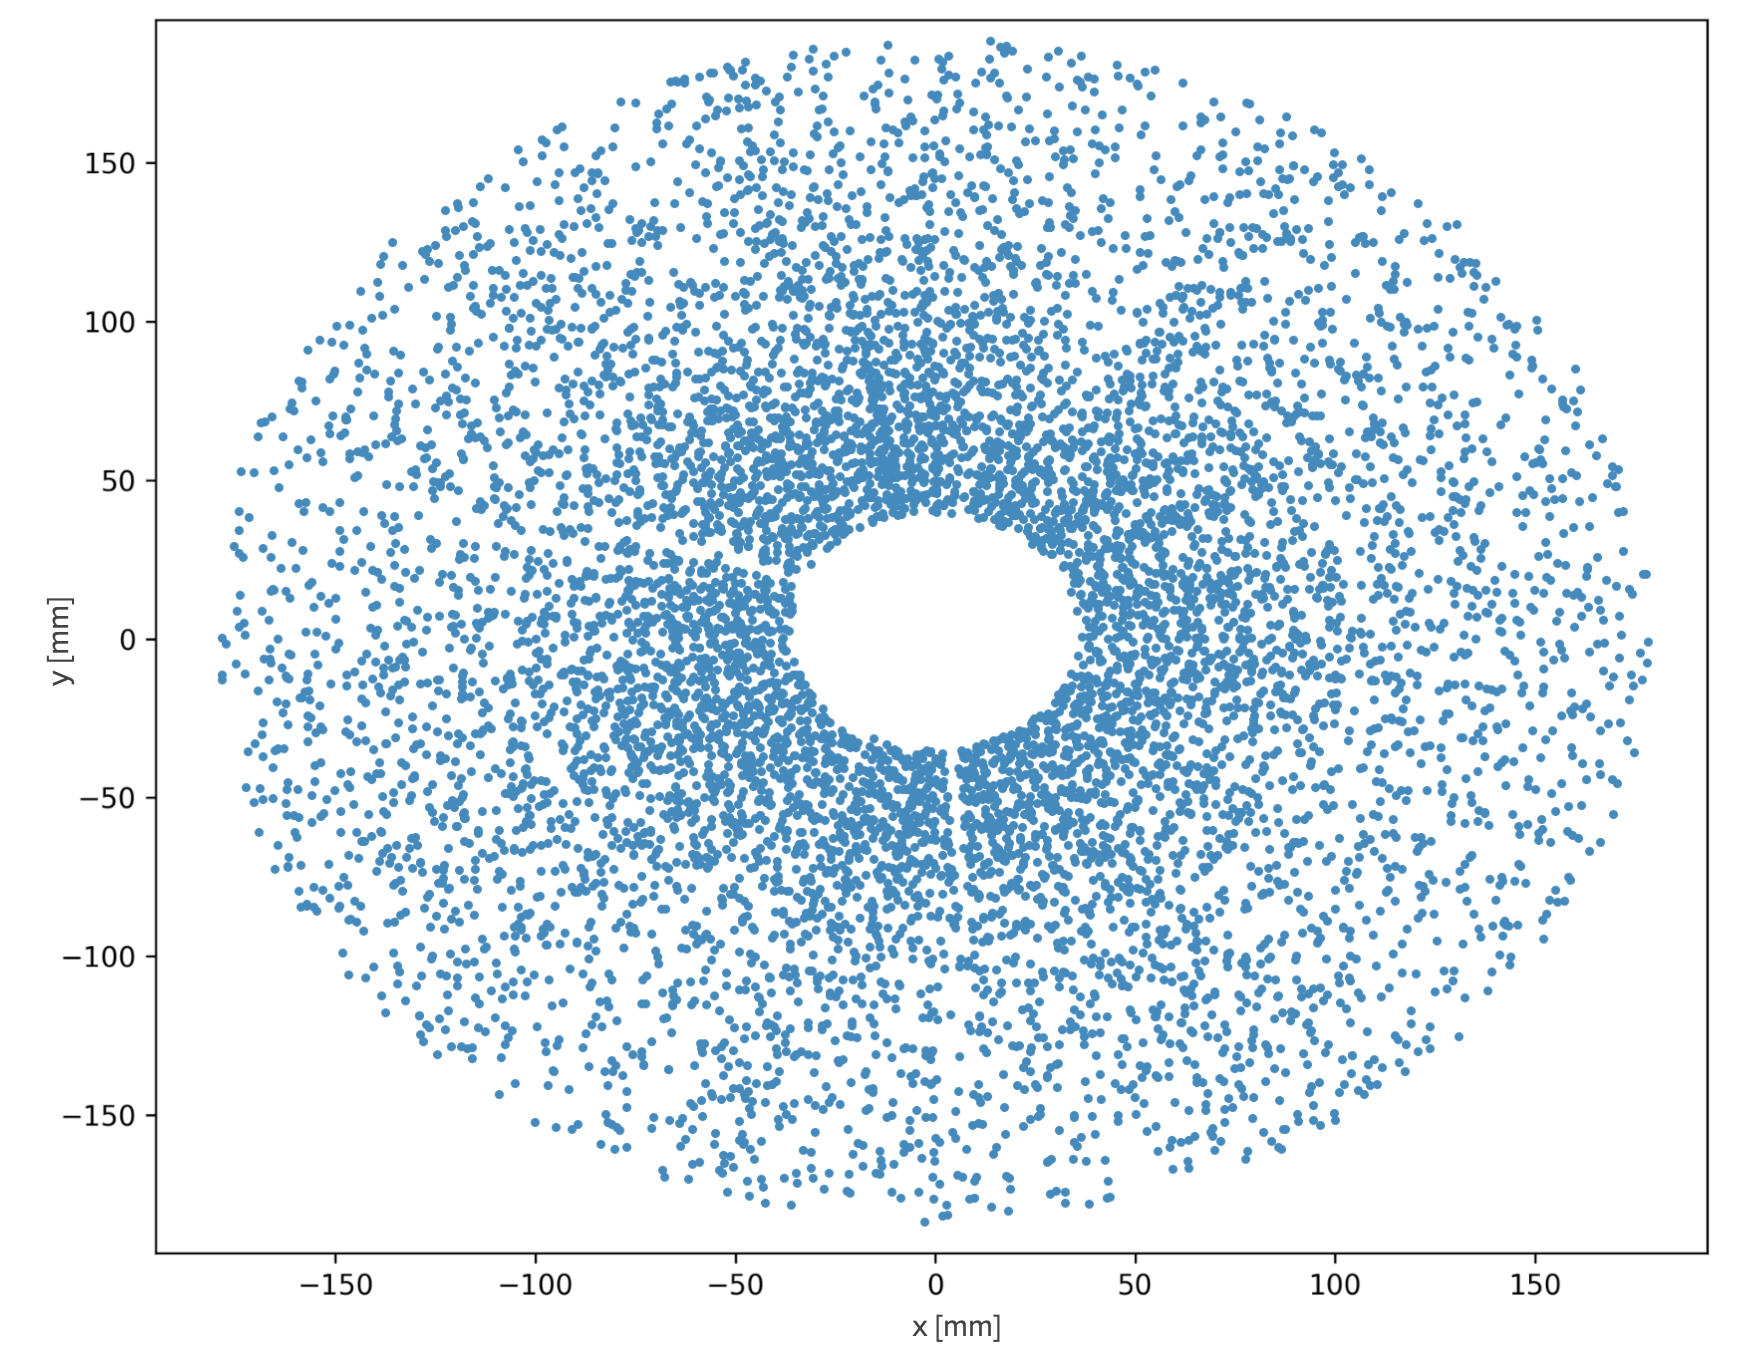
\includegraphics[width=11.5cm]{images/7-results/trackml-endcap-nodes-xy.png} } \label{fig:endcap-trackml-sim-xy}}%
    \hfill
    %\qquad
    \subfloat[\centering ...]{{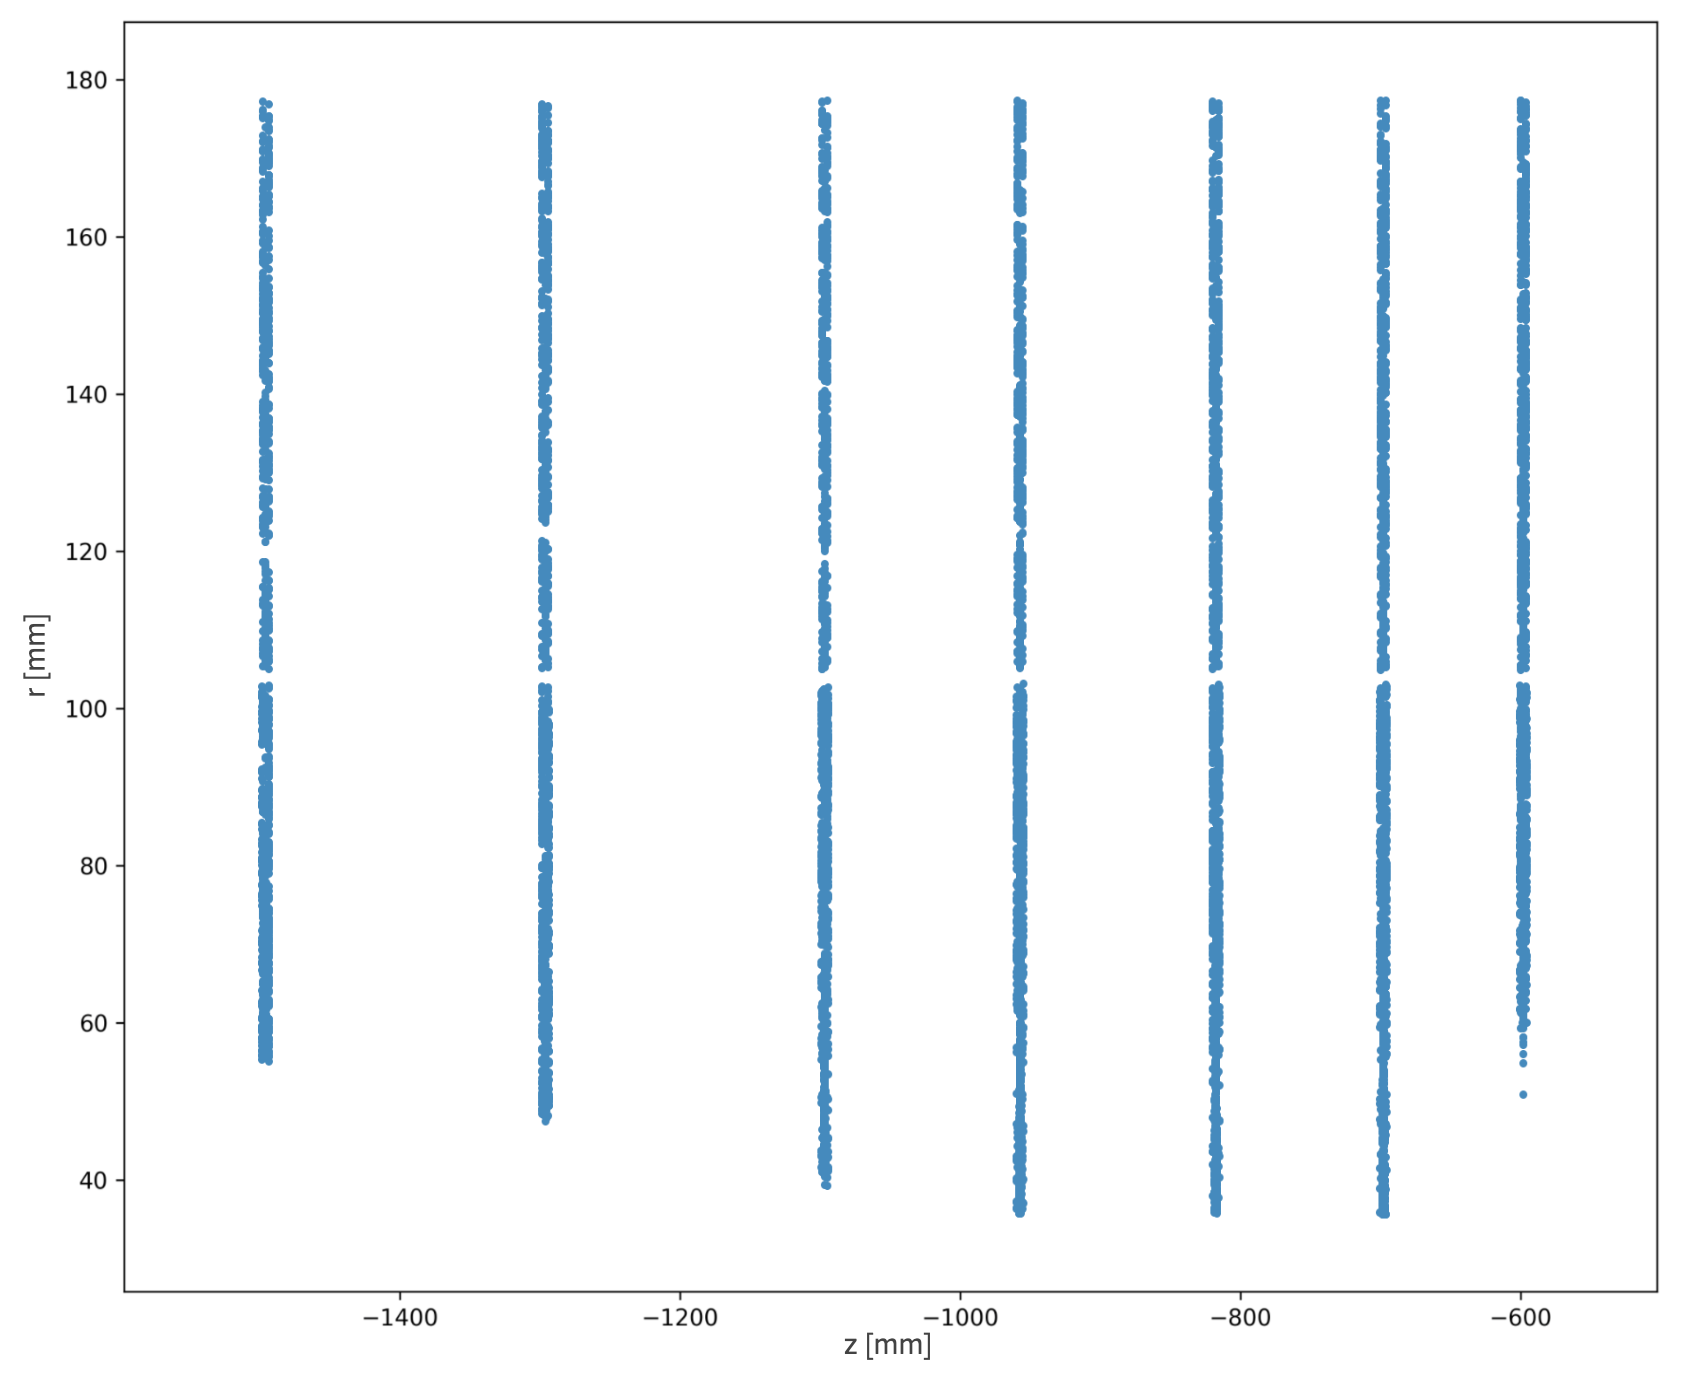
\includegraphics[width=11.5cm]{images/7-results/trackml-endcap-nodes-rz.png} } \label{fig:endcap-trackml-sim-rz}}%
    \caption{....}%
    \label{fig:trackml-results-endcap-nodes-sim}%
\end{figure}



\begin{figure}[htbp]%
    \centering
    \subfloat[\centering ...]{{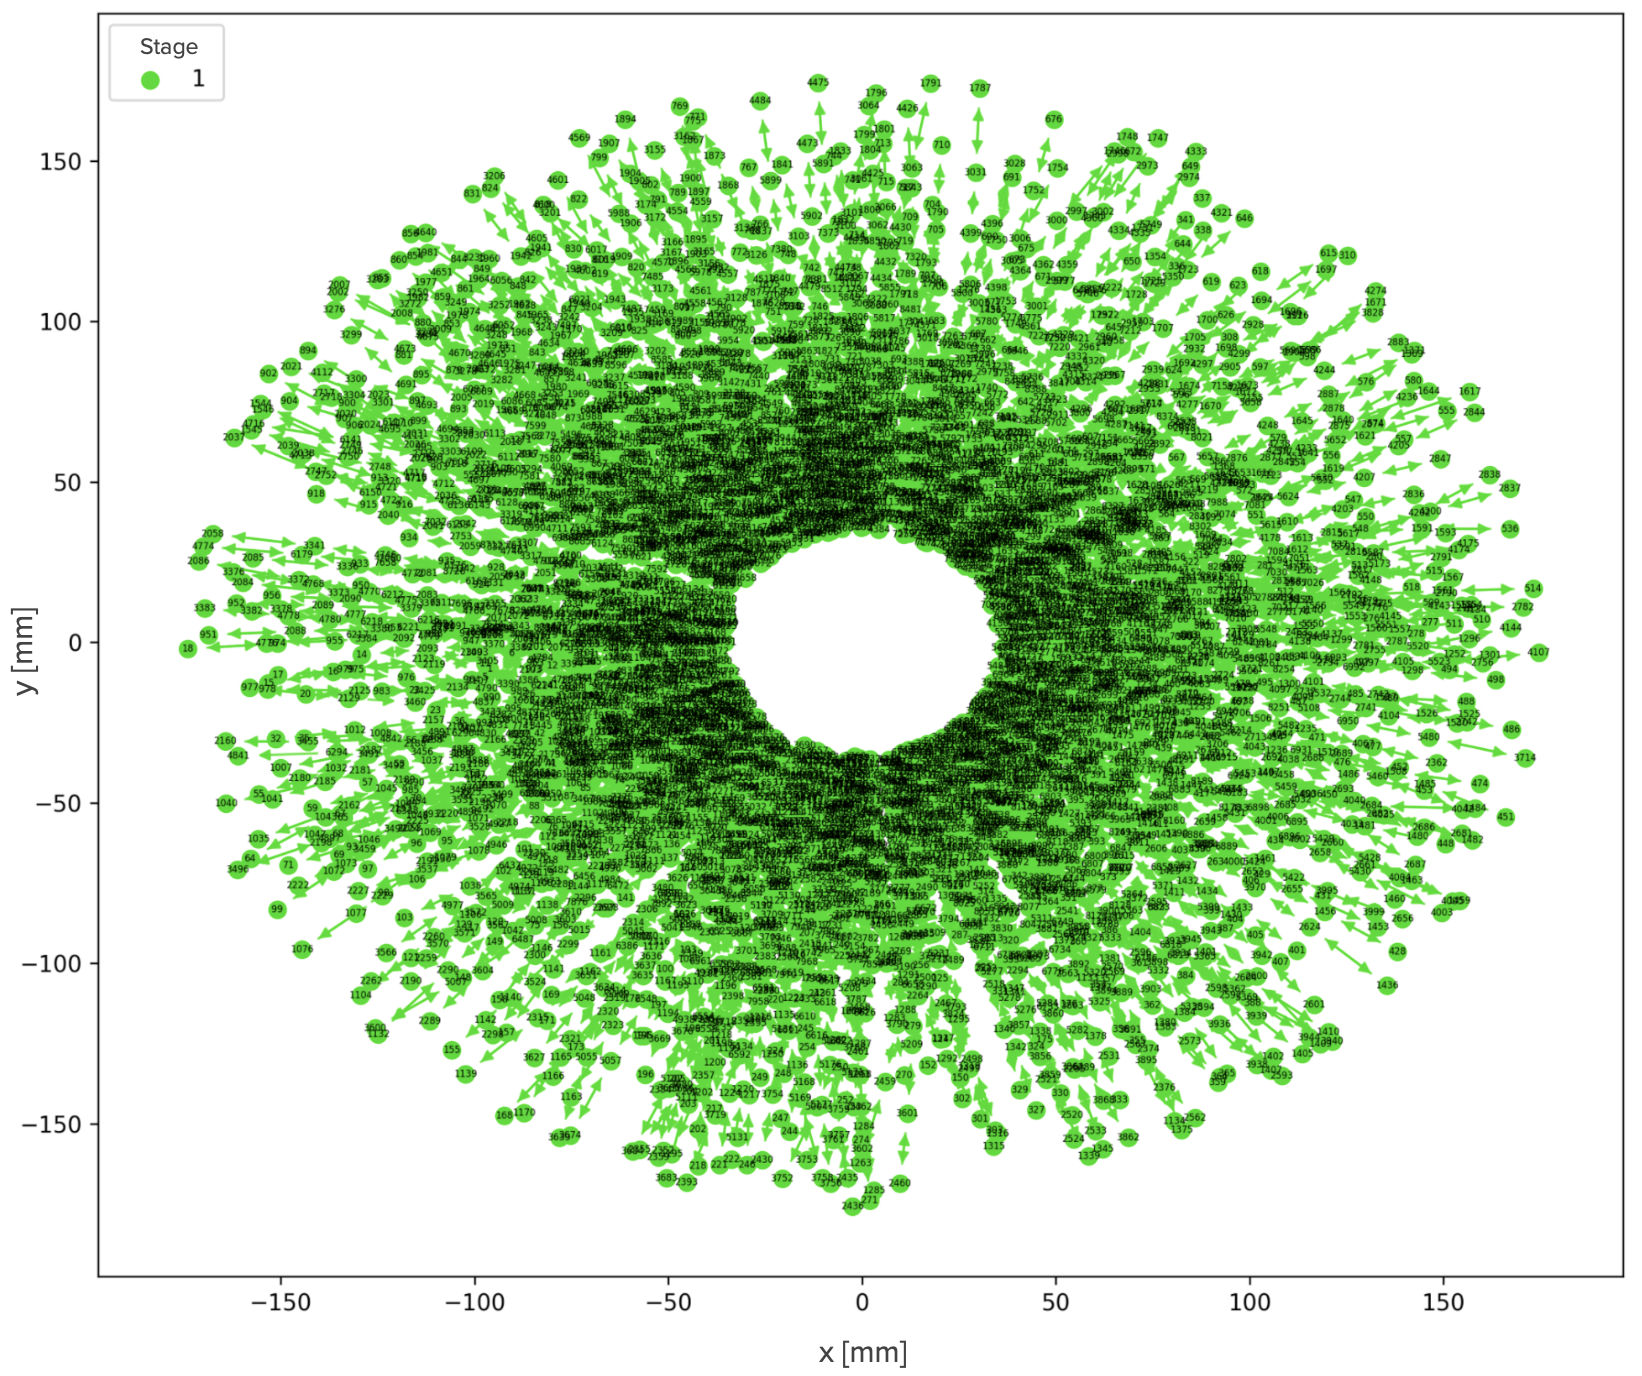
\includegraphics[width=11.5cm]{images/7-results/trackml-endcap-extracted-xy.png} } \label{fig:endcap-trackml-extracted-xy}}%
    \hfill
    %\qquad
    \subfloat[\centering ...]{{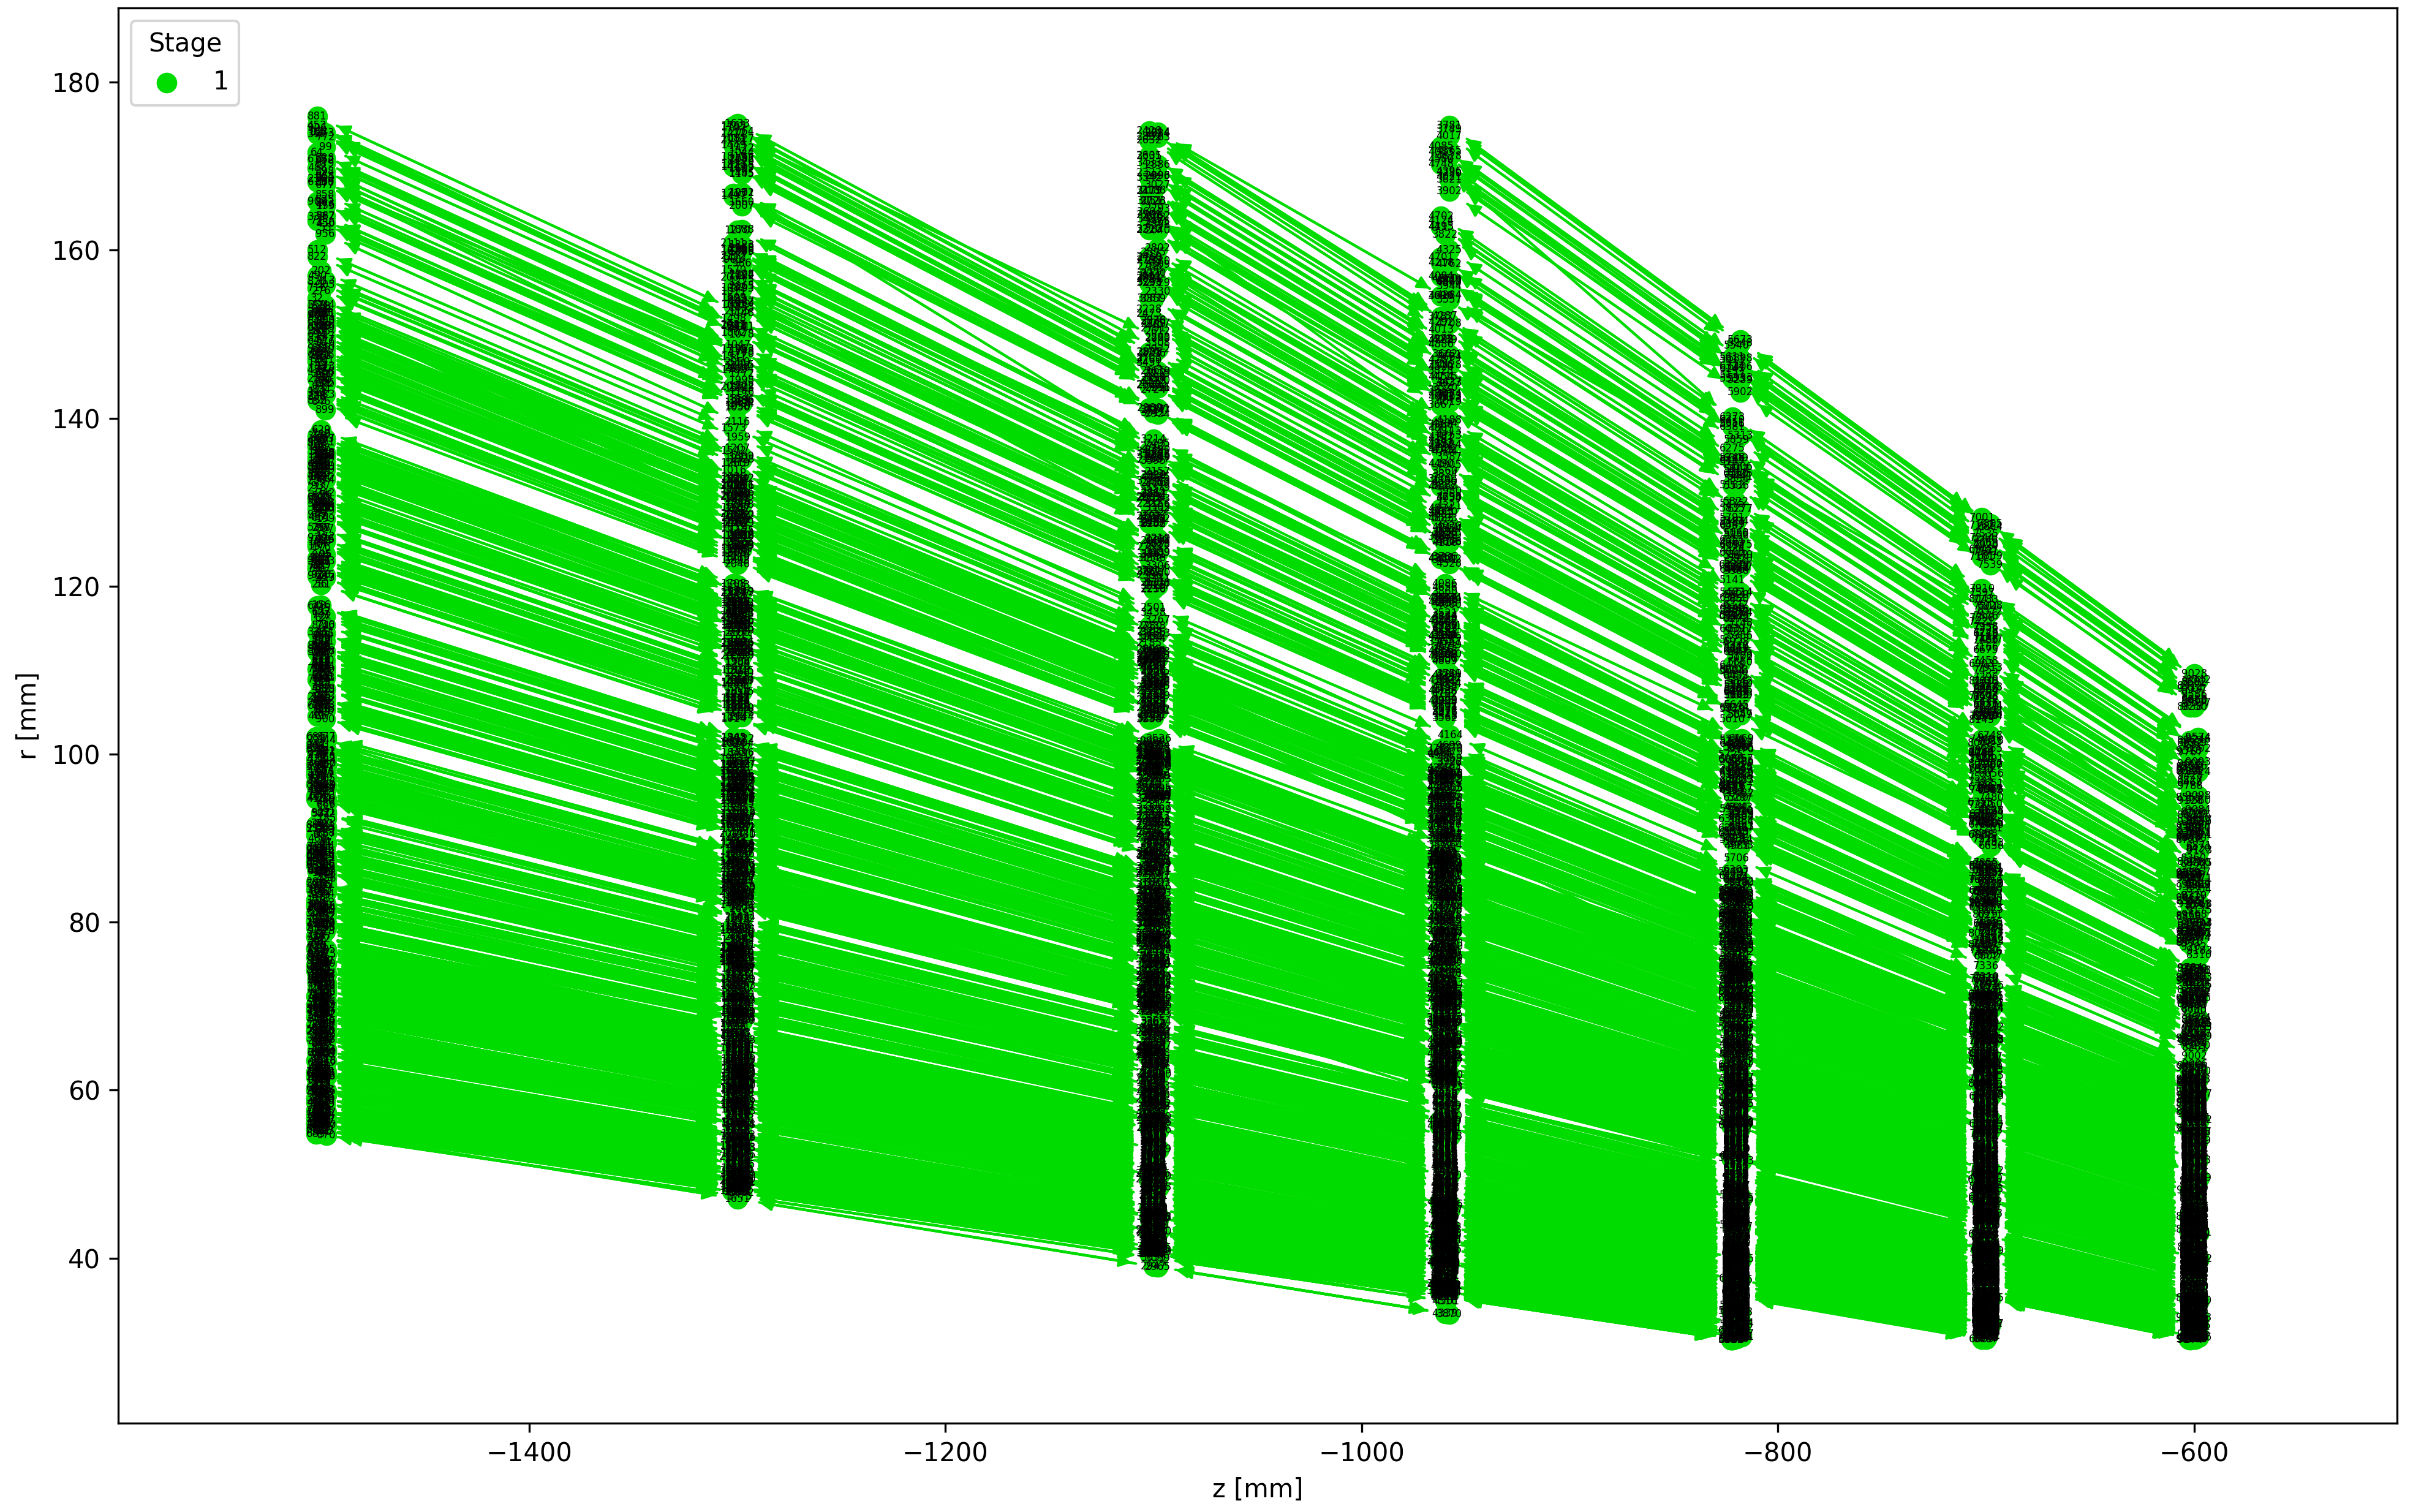
\includegraphics[width=11.5cm]{images/7-results/trackml-endcap-extracted-rz.png} } \label{fig:endcap-trackml-extracted-rz}}%
    \caption{....}%
    \label{fig:trackml-results-endcap-extracted}%
\end{figure}


\begin{figure}[htbp]%
    \centering
    \subfloat[\centering ...]{{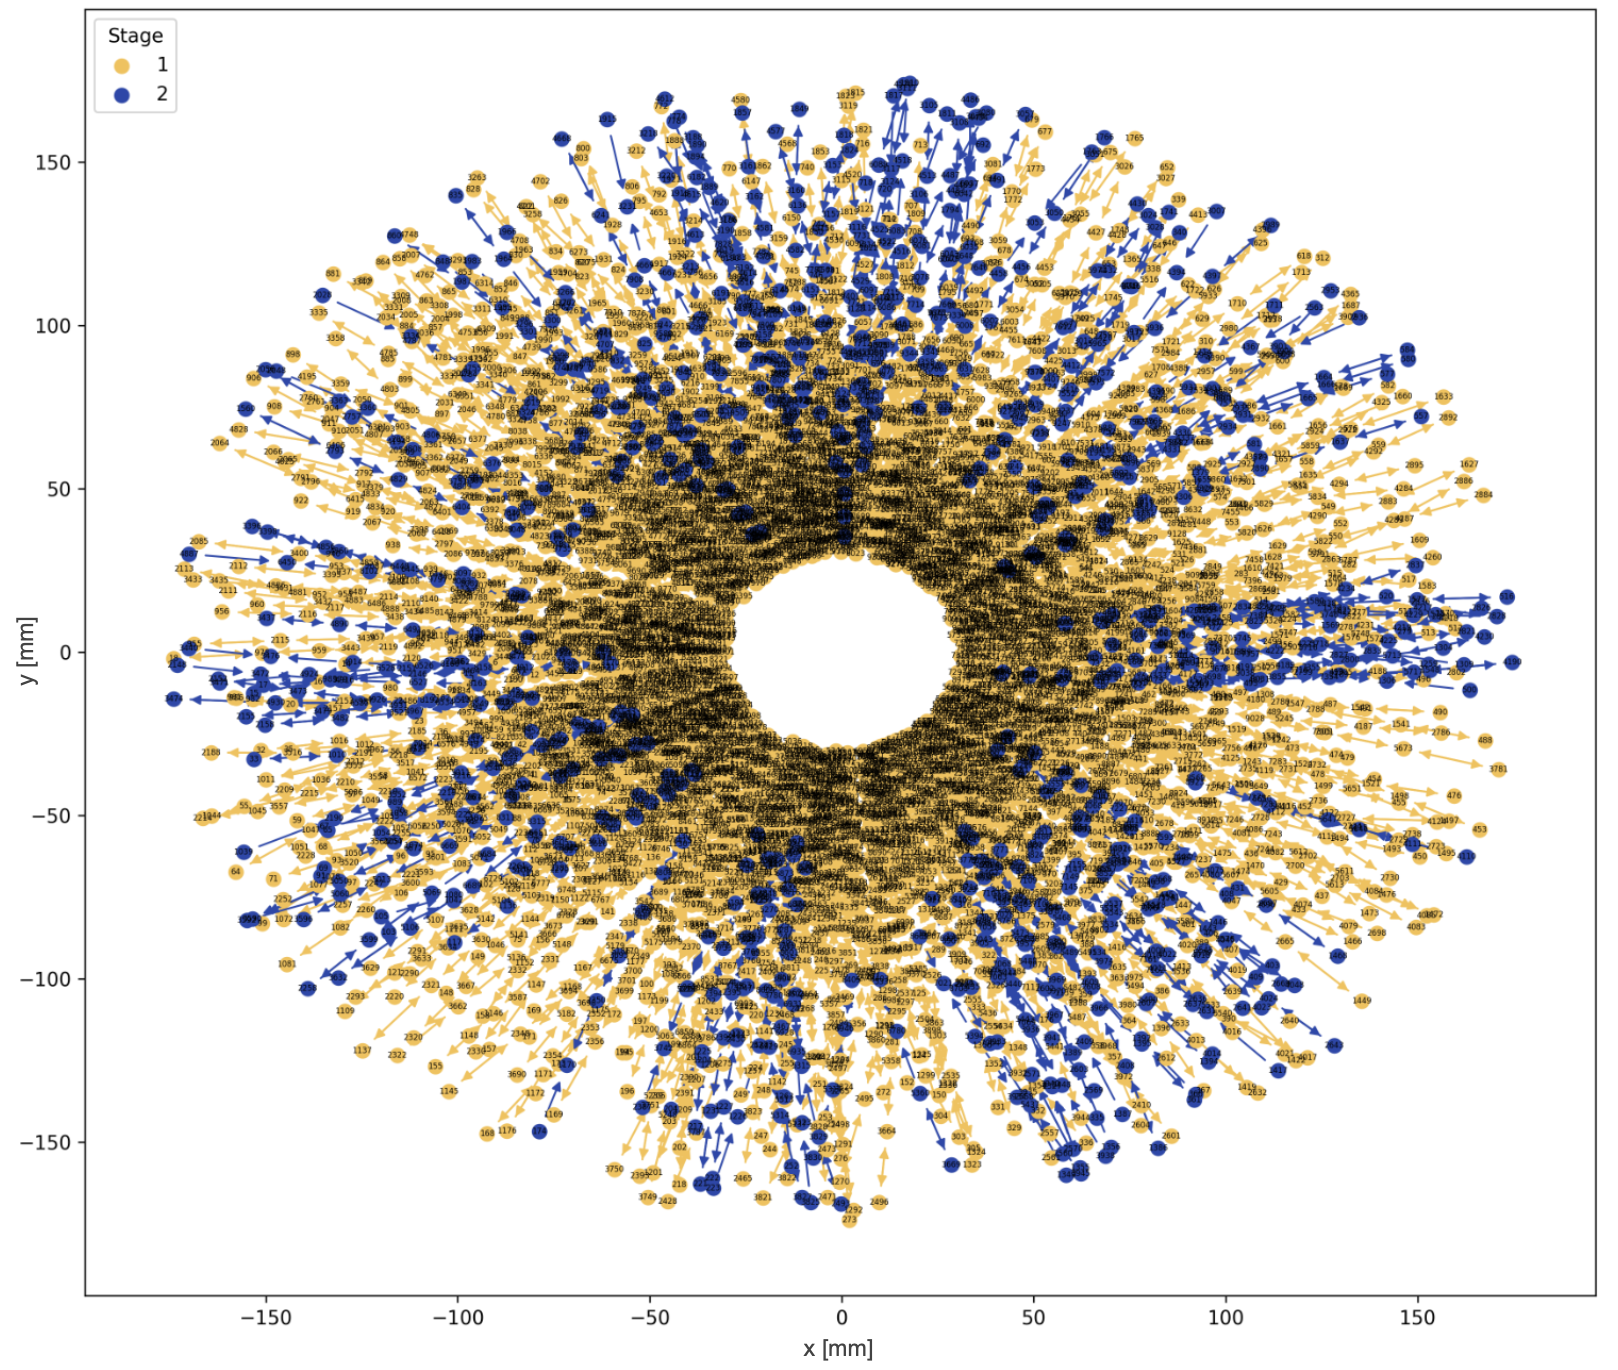
\includegraphics[width=11.5cm]{images/7-results/trackml-endcap-extracted-xy-v2.png} } \label{fig:endcap-trackml-extracted-xy-v2}}%
    \hfill
    %\qquad
    \subfloat[\centering ...]{{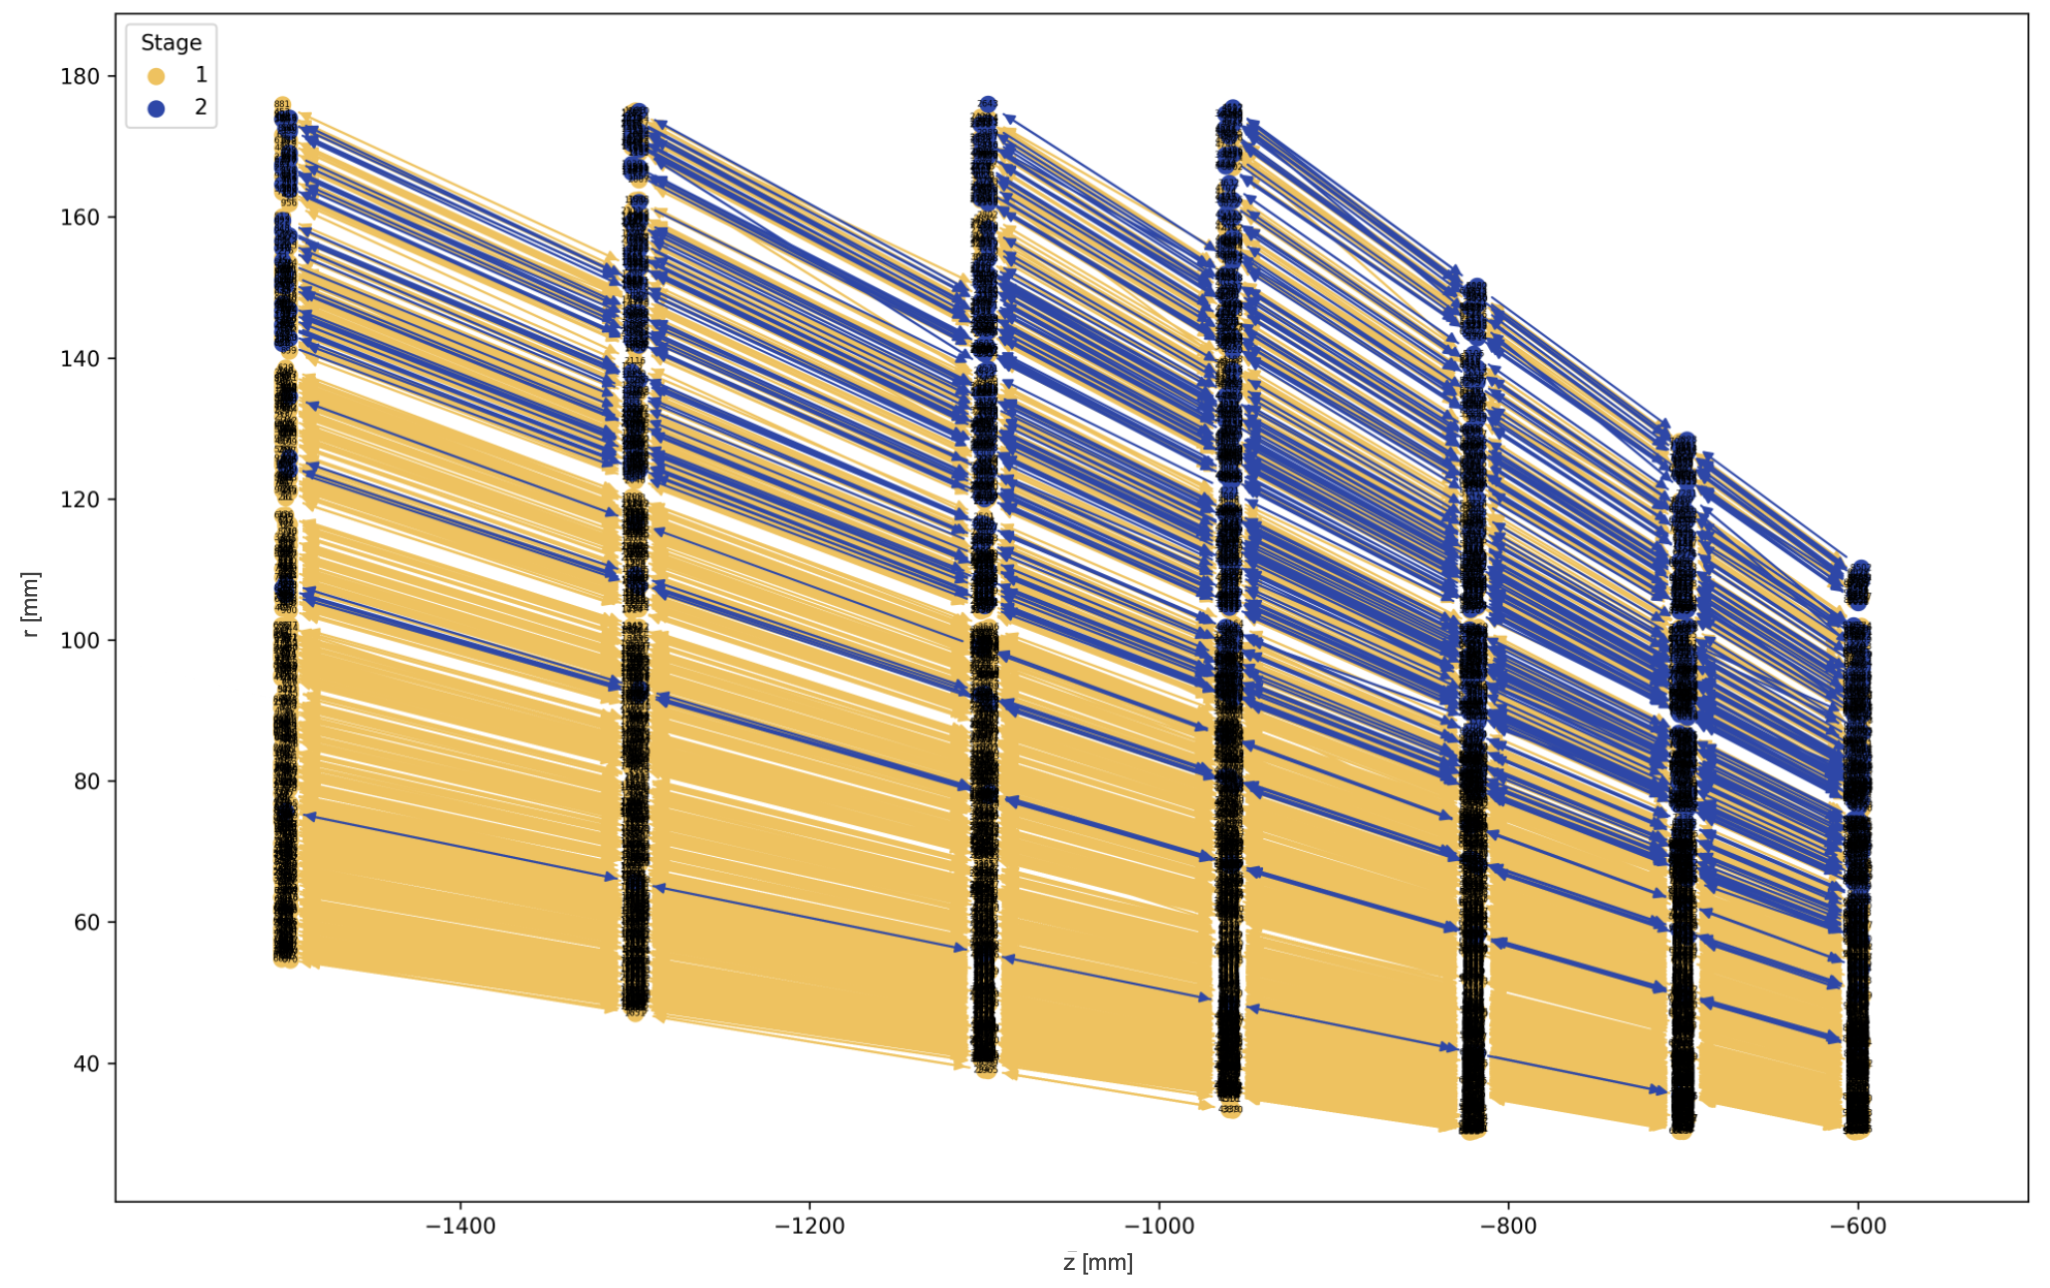
\includegraphics[width=14cm]{images/7-results/trackml-endcap-extracted-rz-v2.png} } \label{fig:endcap-trackml-extracted-rz-v3}}%
    \caption{....}%
    \label{fig:trackml-results-endcap-extracted-v2}%
\end{figure}





% TODO: one more example of the endcap on its own, but this time with more than 1 stage of the algorithm shown

% TODO: in the performance evaluation section --> need an average of results over many events executed



\subsection{Performance Evaluation}

\begin{figure}[htbp]
    \centering
    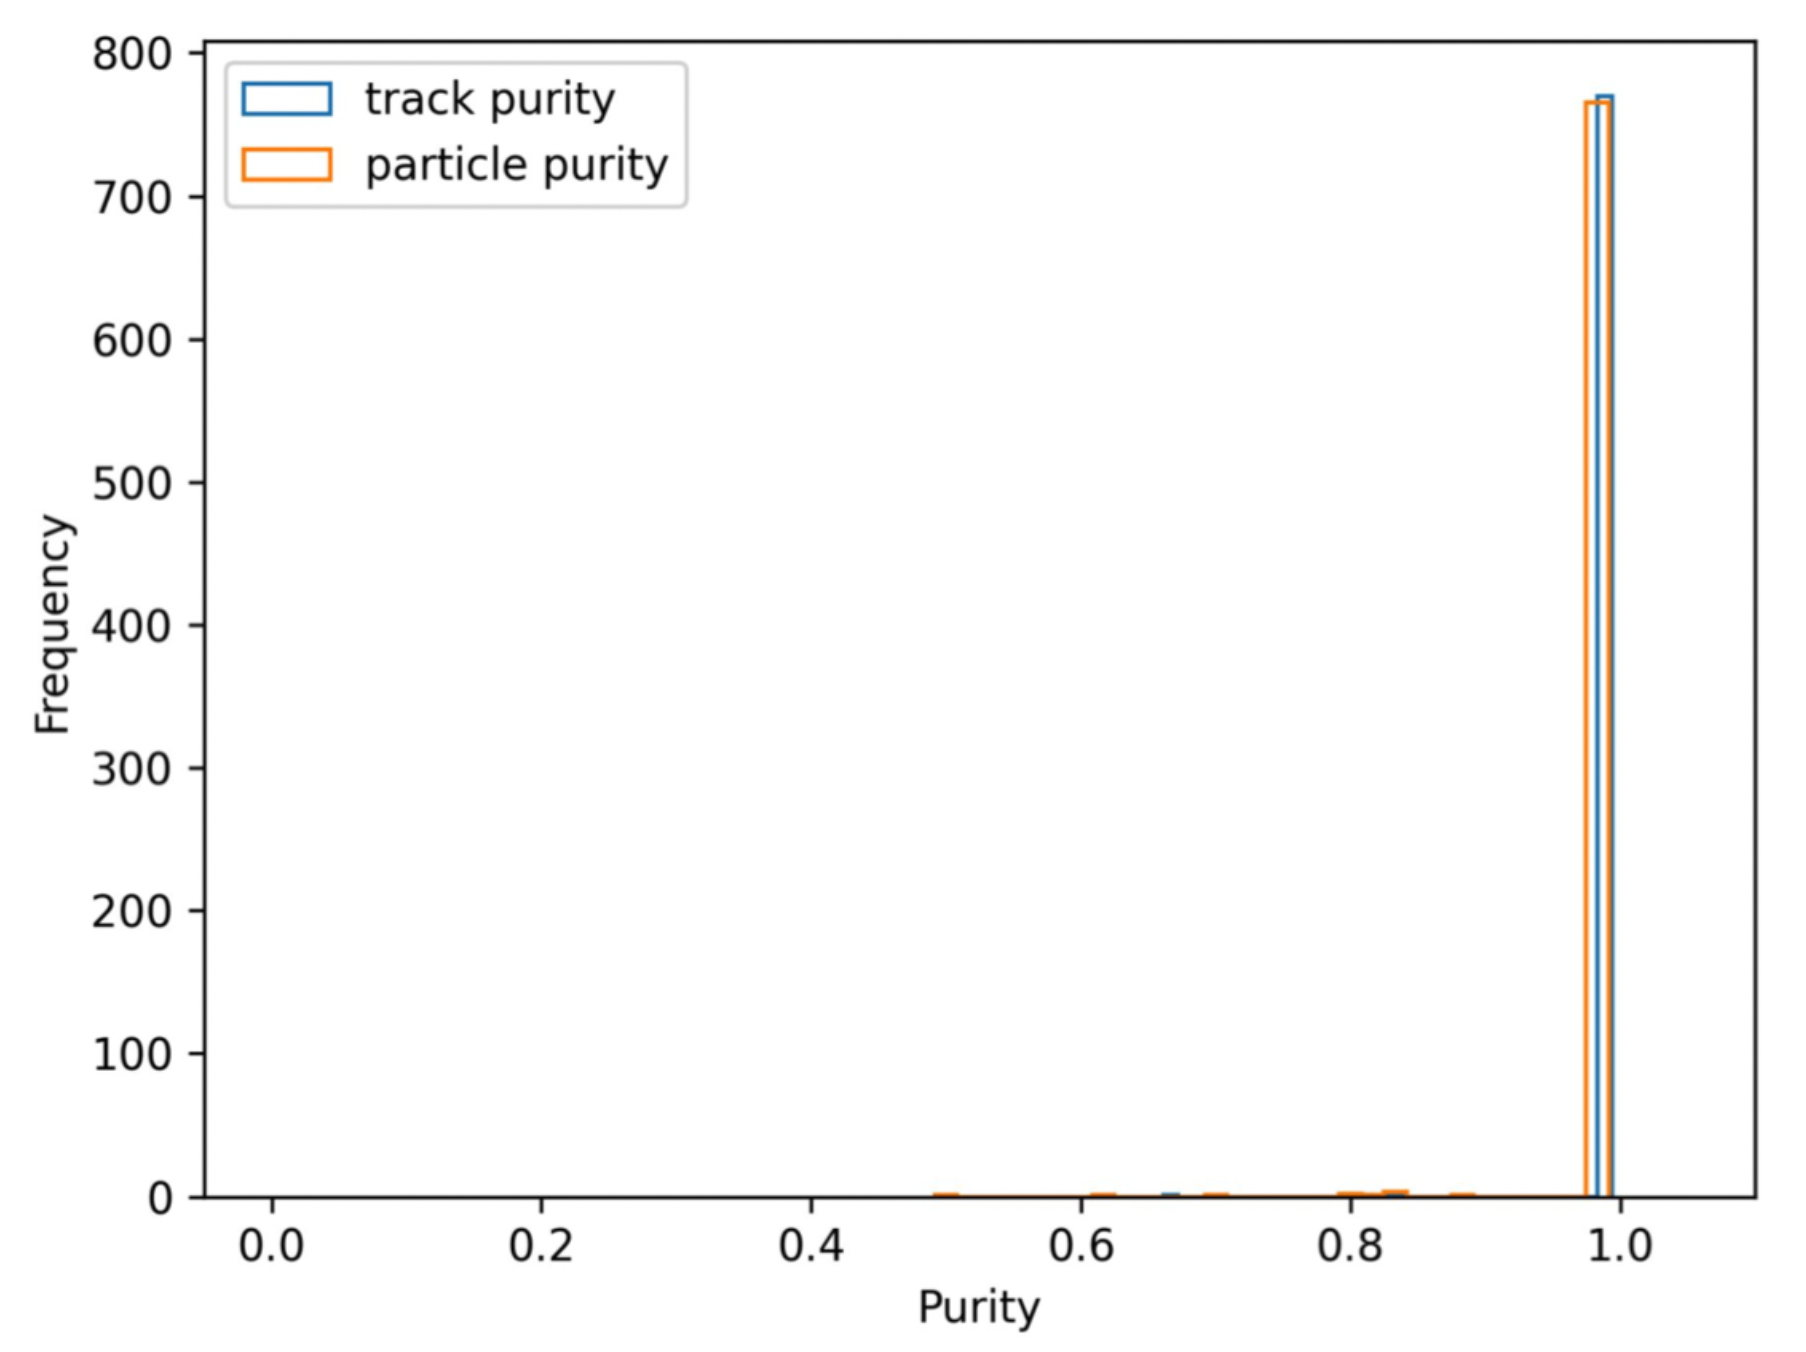
\includegraphics[width=0.7\textwidth]{images/7-results/endcap-purity.png}
    \caption{...}
    \label{fig:trackml-results-endcap-nodes-purity}%
\end{figure}


% track purity, particle purity, track reconstruction efficiency
% TODO: mention here that the parabolic track state model was used and the joint track state was used, and mention the section here

%nips-2018-competation
%Data.
%We used the fast (10s per event) and accurate simulation engine ACTS4 [6] to generate the challenge data. It allowed us to generate realistic data emulating a full Silicon LHC detector (see Fig 3), while providing us with the ground truth of particle trajectory membership. Thus, for each event we obtained the “detected” 3D points coordinates (and additional features), and, as ground truth, the list of points associated to each track. There is a one to one relationship between the true 3D points and the reconstructed ones.

%\begin{itemize}
%    \item Application on TrackML model, endcap volume only, metrics, performance eval etc, track reconstruction efficiency, track purity and particle purity, comparison with TrackML solutions
%    \item Track reconstruction efficiency, track purity, particle purity
%    \item Performance Evaluation
%    \item execution time?
%\end{itemize}

% need to present the average over many events here



% Importance of KF application:
%An important aspect of the application of the KF here is that reconstruction of curved tracks is possible using a low-dimensionality model. By assuming a slow change in track direction, a special dynamic model for the KF is constructed using the OU process, which implicitly takes into account the track curvature without extending the track state with additional parameters.



\section{Outlook}
\label{chapter-7-outlook}

\subsection{Extension to the Pixel Barrel Region}

% \begin{figure}[htbp]
%     \centering
%     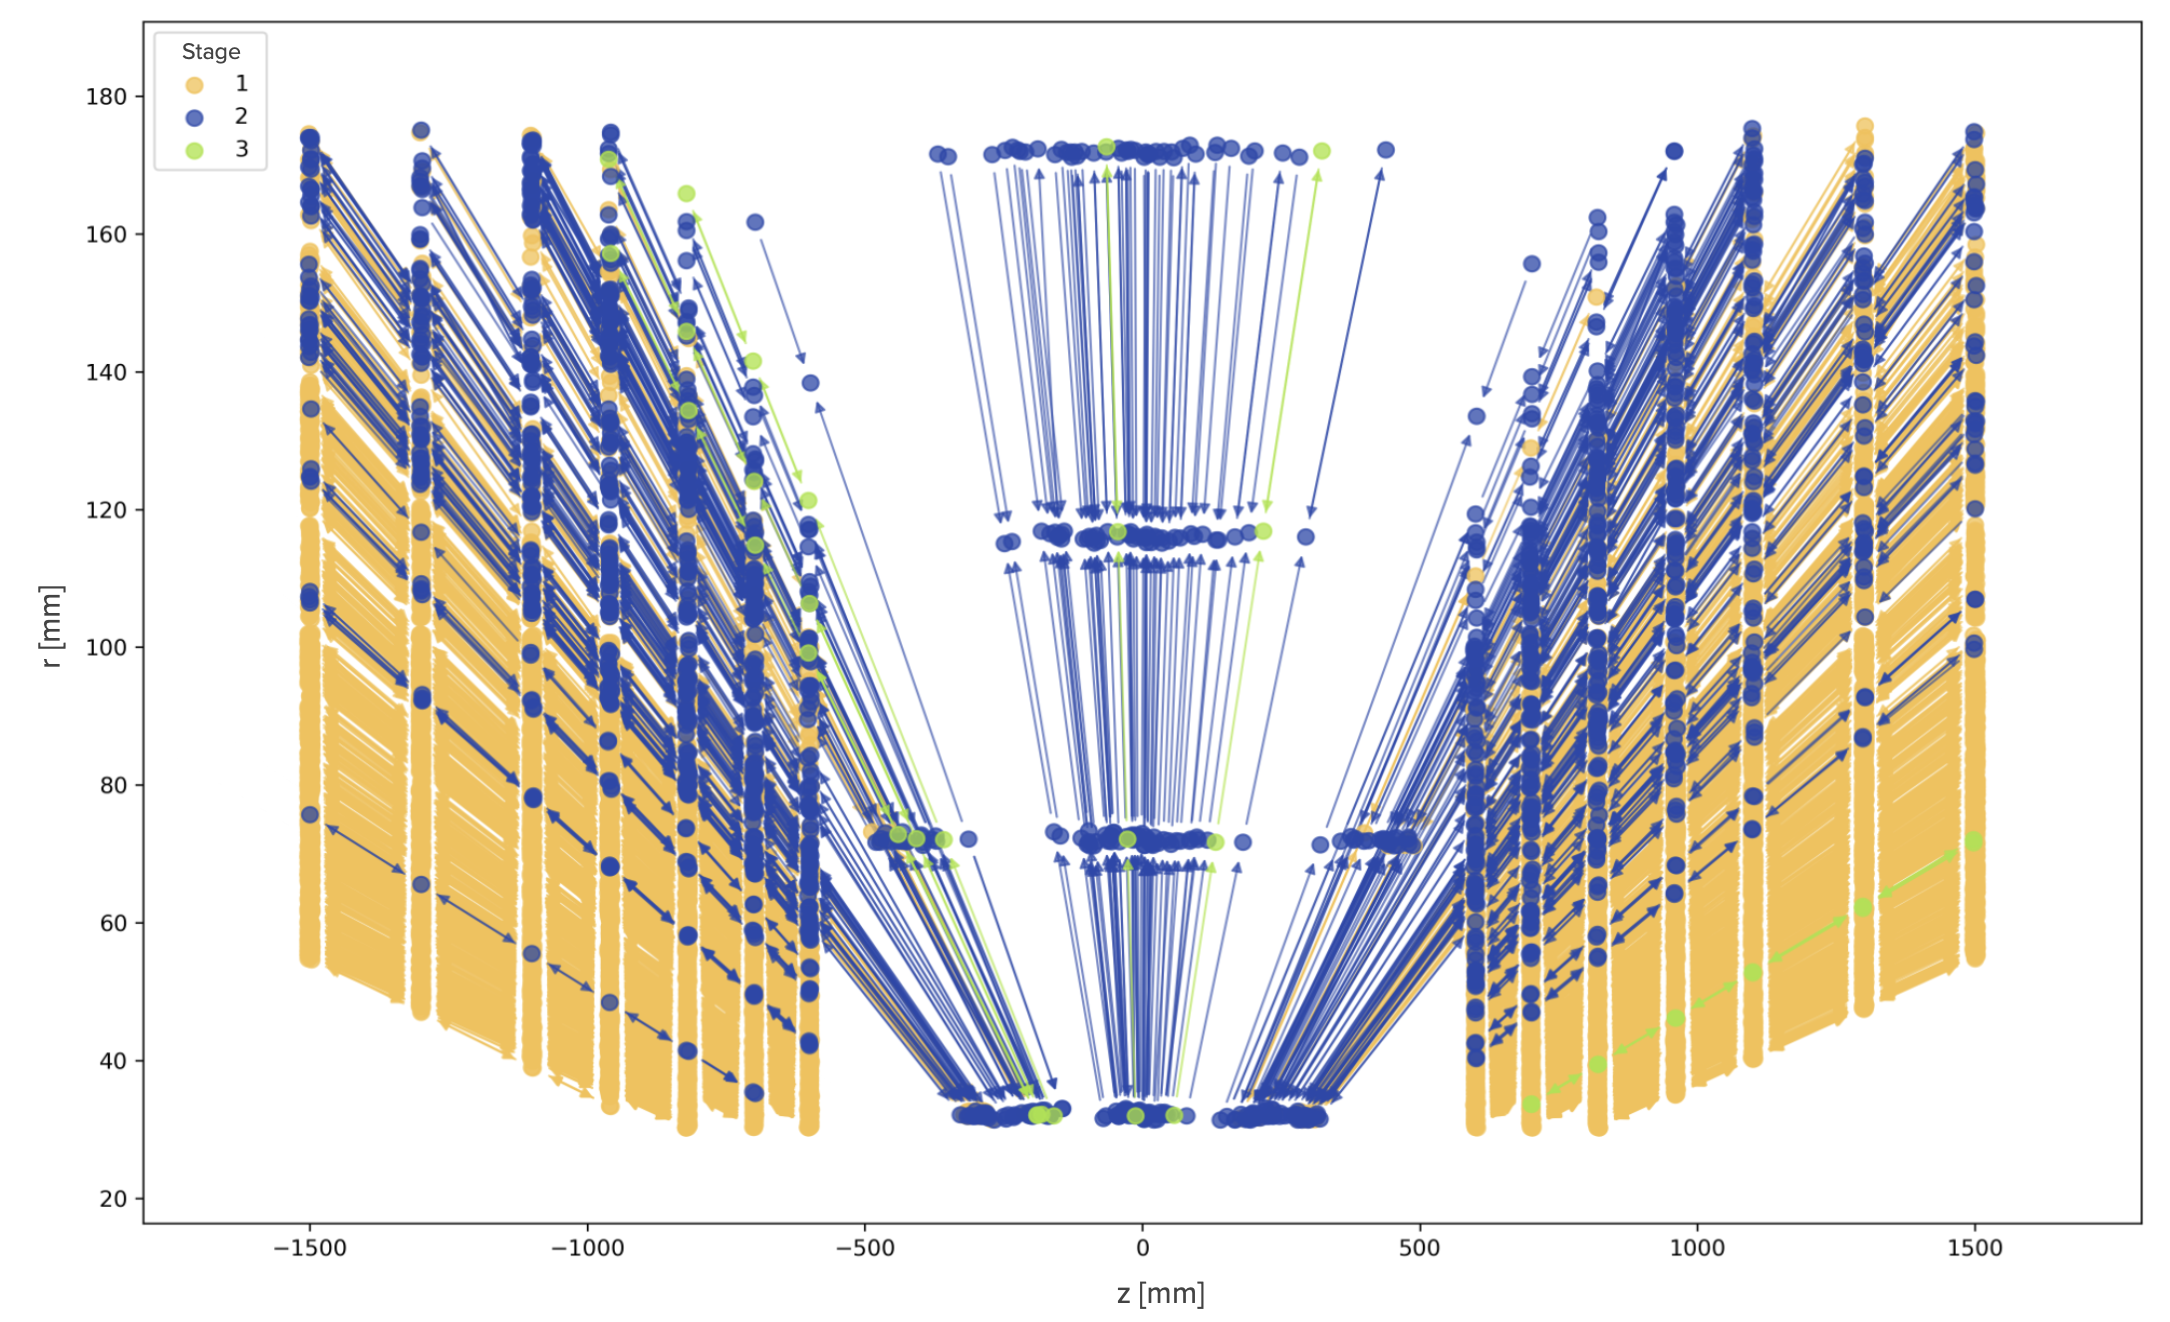
\includegraphics[width=0.99\textwidth]{images/7-results/trackml-endcap-barrel-results.png}
%     \caption{...}
%     \label{fig:trackml-results-barrel-endcap}%
% \end{figure}


\begin{figure}[htbp]%
    \centering
    \subfloat[\centering ...]{{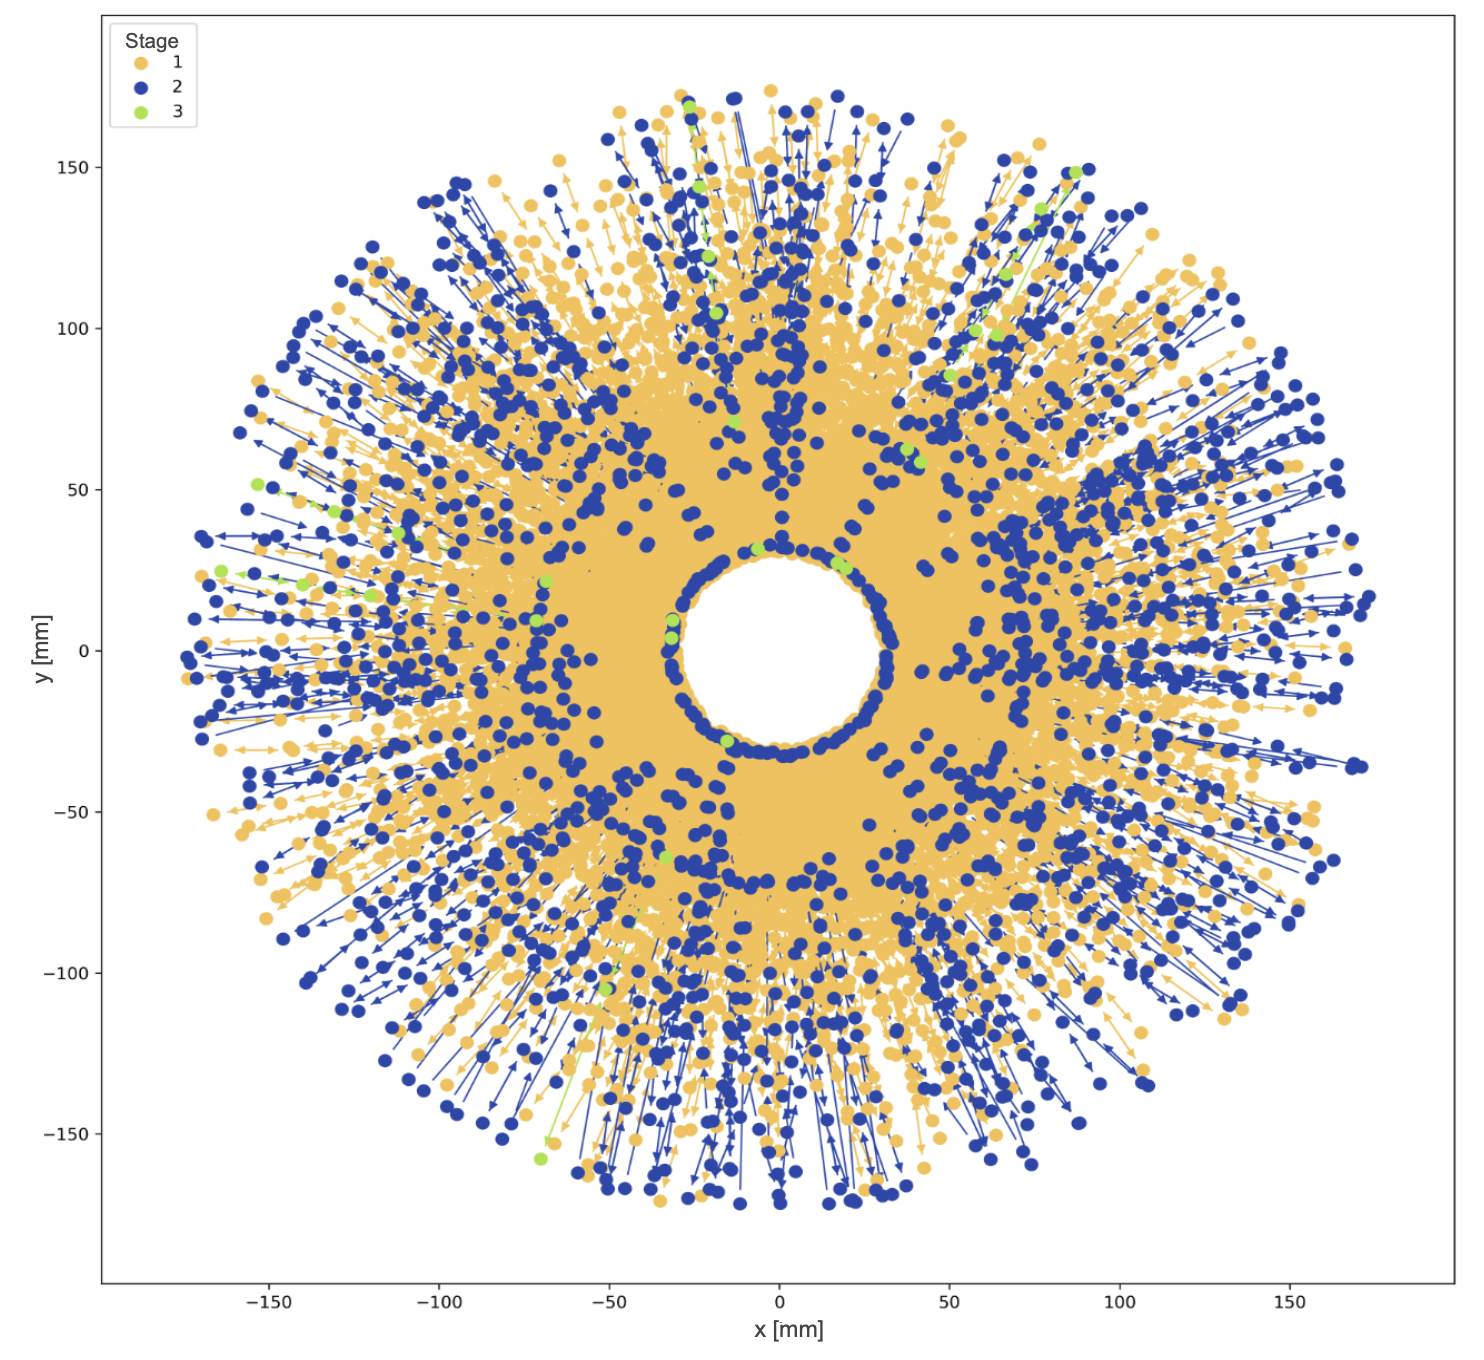
\includegraphics[width=10cm]{images/7-results/trackml-endcap-barrel-extracted-xy.png} } \label{fig:trackml-results-barrel-endcap-extracted-xy}}%
    \hfill
    %\qquad
    \subfloat[\centering ...]{{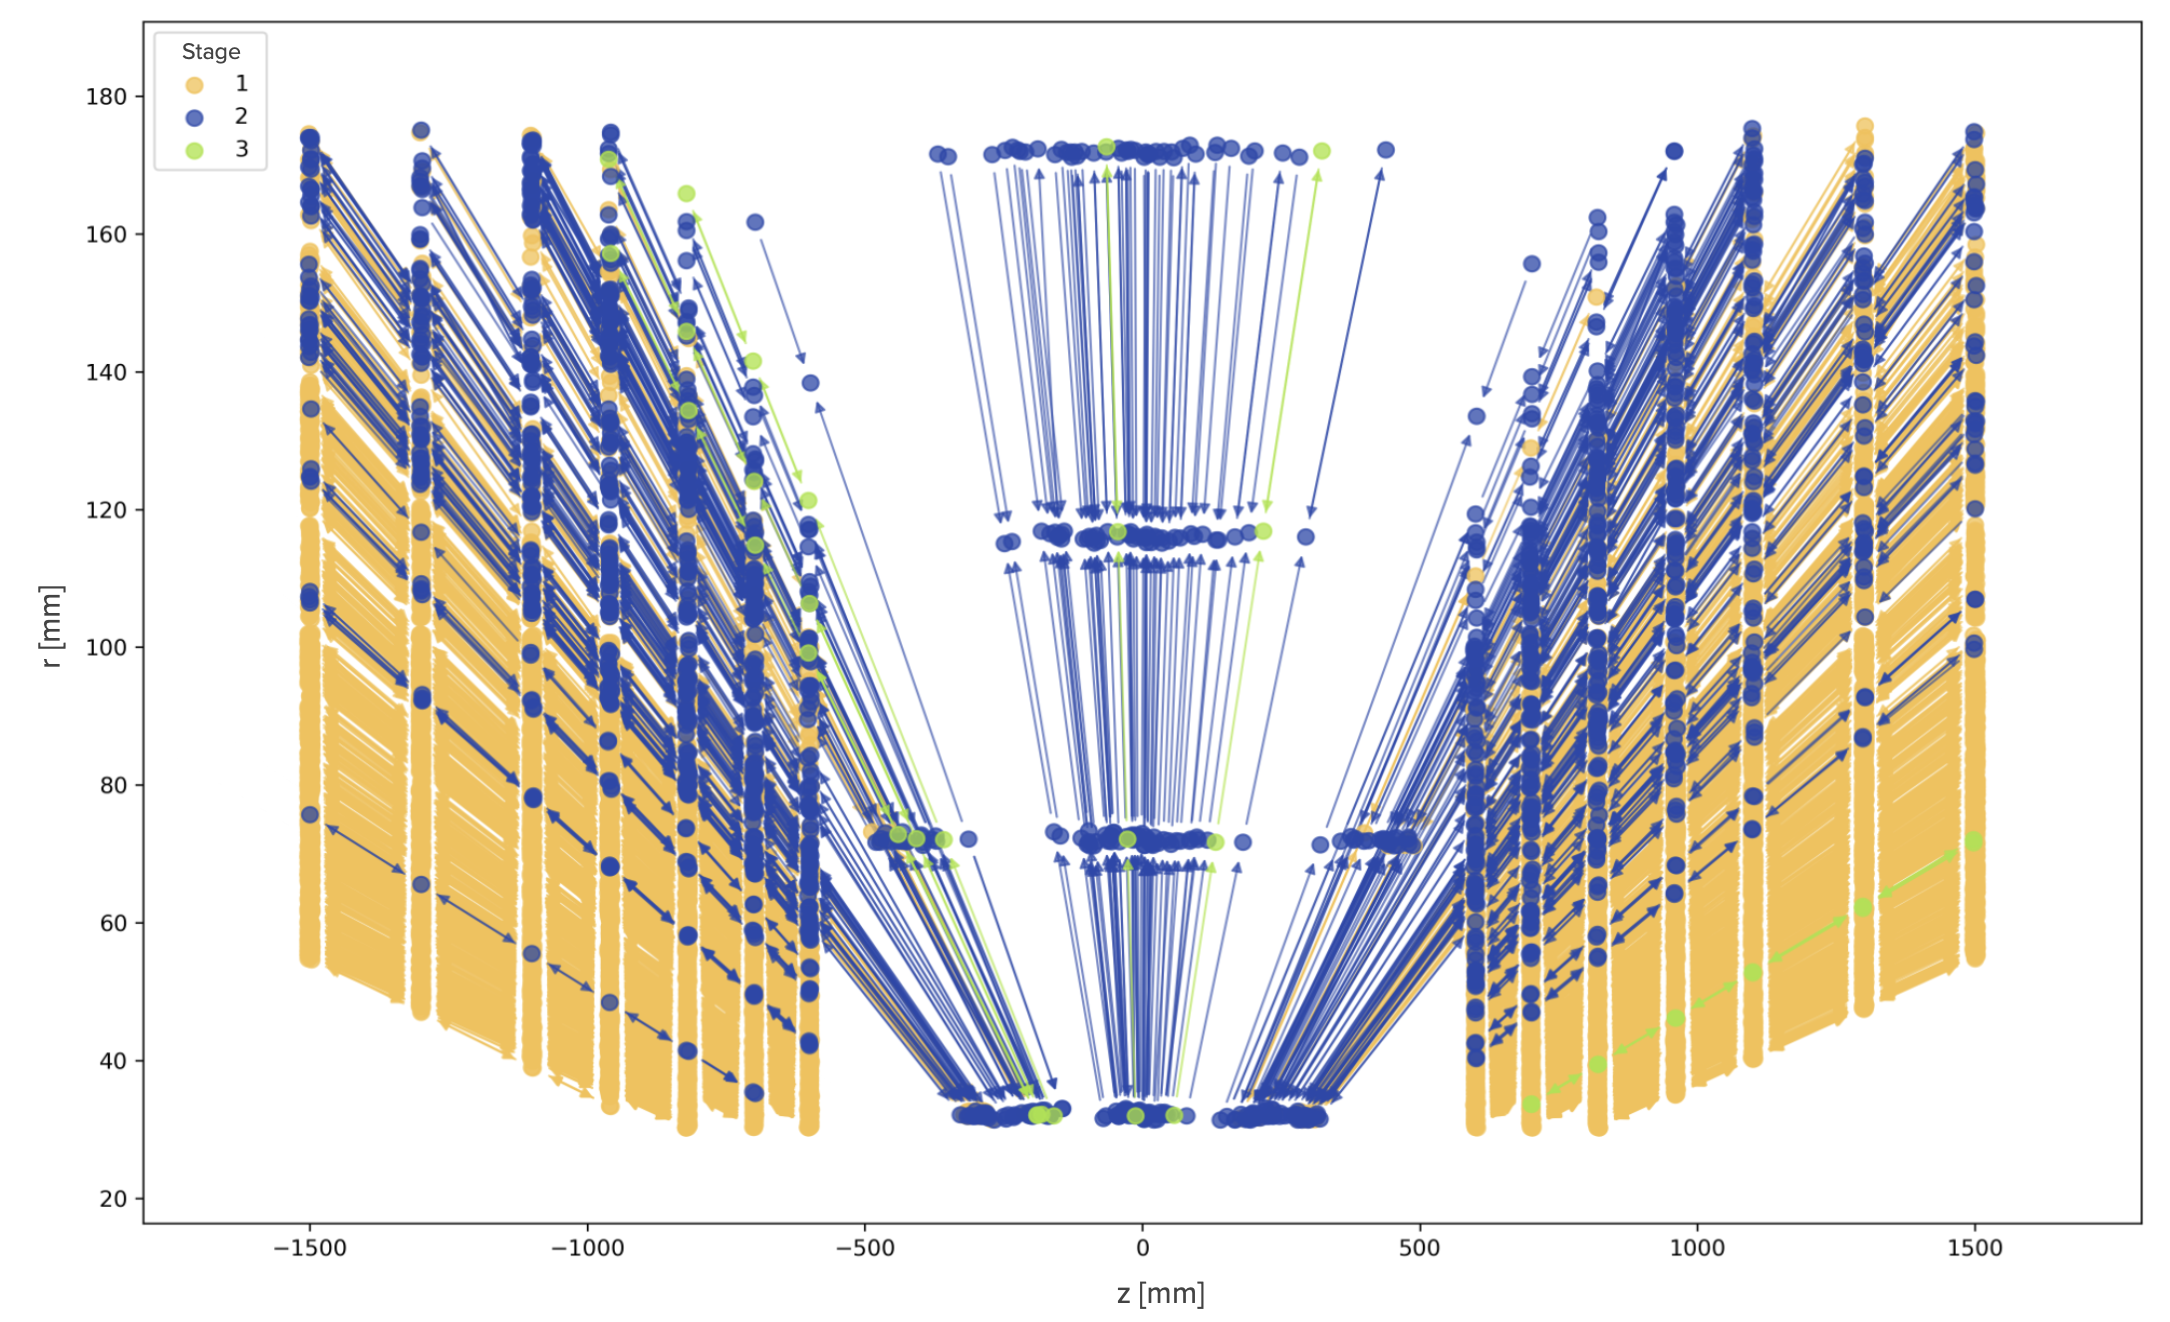
\includegraphics[width=14cm]{images/7-results/trackml-endcap-barrel-extracted-rz.png} } \label{fig:trackml-results-barrel-endcap-extracted-rz}}%
    \caption{....}%
    \label{fig:trackml-results-barrel-endcap}%
\end{figure}










\begin{figure}[htbp]
    \centering
    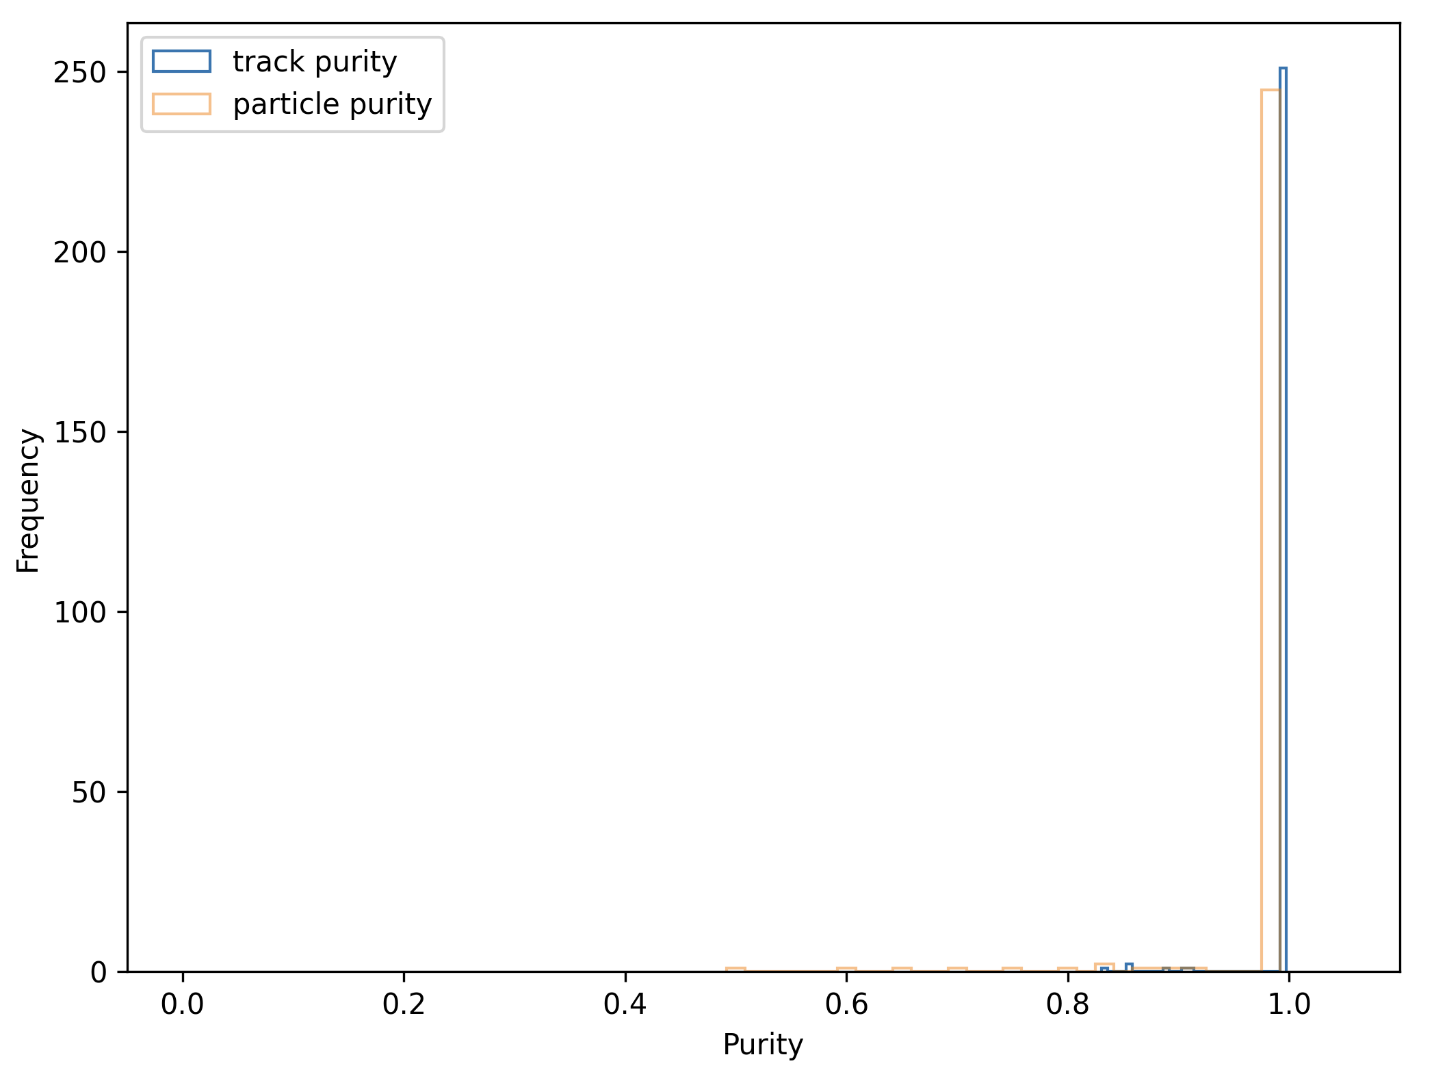
\includegraphics[width=0.7\textwidth]{images/7-results/barrel-and-endcap-purity.png}
    \caption{...}
    \label{fig:trackml-results-barrel-endcap-purity}%
\end{figure}


% confusion matrices for barrel and endap, stages 1 and 2
\begin{figure}
    \centering
    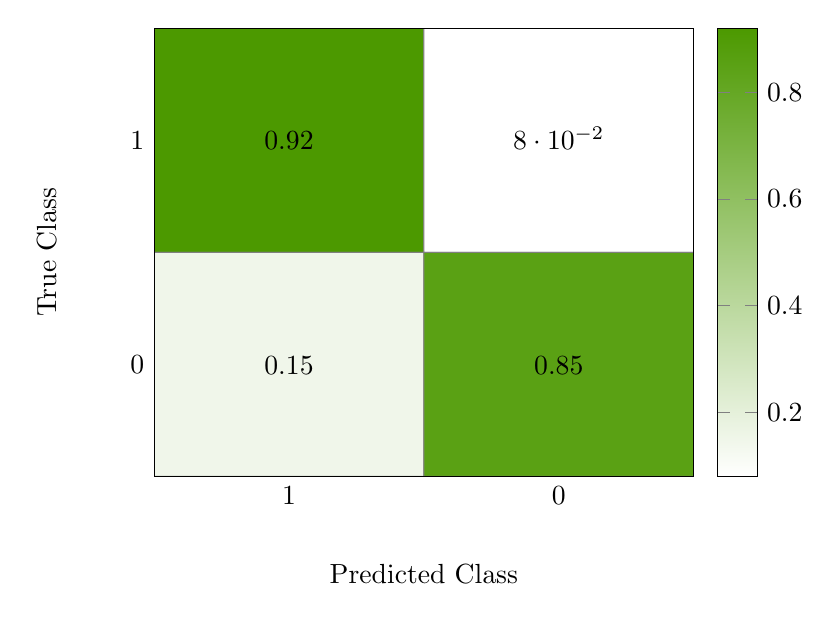
\begin{tikzpicture}
        \begin{axis}[
                colormap={greenyellow}{color=(white) rgb255=(76,153,0)},
                xlabel=Predicted Class,
                xlabel style={yshift=-15pt},
                ylabel=True Class,
                ylabel style={yshift=20pt},
                xticklabels={1, 0}, % changed
                xtick={0,...,1}, % changed
                xtick style={draw=none},
                yticklabels={1, 0}, % changed
                ytick={0,...,1}, % changed
                ytick style={draw=none},
                enlargelimits=false,
                colorbar,
                xticklabel style={rotate=0},
                nodes near coords={\pgfmathprintnumber\pgfplotspointmeta},
                nodes near coords style={yshift=-7pt},
            ]
            \addplot[
                matrix plot,
                mesh/cols=2, % changed
                point meta=explicit,draw=gray
            ] table [meta=C] {
                x y C
                0 0 0.92
                1 0 0.08     
                0 1 0.15
                1 1 0.85
            };
        \end{axis}
    \end{tikzpicture}
    \caption{TODO...Stage 1 confusion matrix}
    \label{fig:confusion-matrix-barrel-endcap-stage-1}
\end{figure}


\begin{figure}
    \centering
    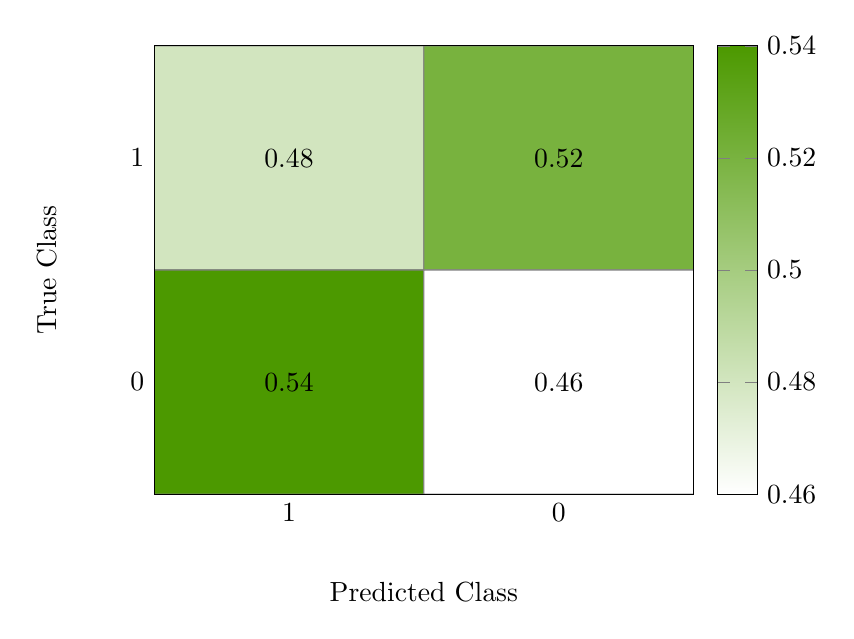
\begin{tikzpicture}
        \begin{axis}[
                colormap={greenyellow}{color=(white) rgb255=(76,153,0)},
                xlabel=Predicted Class,
                xlabel style={yshift=-15pt},
                ylabel=True Class,
                ylabel style={yshift=20pt},
                xticklabels={1, 0}, % changed
                xtick={0,...,1}, % changed
                xtick style={draw=none},
                yticklabels={1, 0}, % changed
                ytick={0,...,1}, % changed
                ytick style={draw=none},
                enlargelimits=false,
                colorbar,
                xticklabel style={rotate=0},
                nodes near coords={\pgfmathprintnumber\pgfplotspointmeta},
                nodes near coords style={yshift=-7pt},
            ]
            \addplot[
                matrix plot,
                mesh/cols=2, % changed
                point meta=explicit,draw=gray
            ] table [meta=C] {
                x y C
                0 0 0.48
                1 0 0.52     
                0 1 0.54
                1 1 0.46
            };
        \end{axis}
    \end{tikzpicture}
    \caption{TODO...Stage 2 confusion matrix}
    \label{fig:confusion-matrix-barrel-endcap-stage-2}
\end{figure}












\begin{figure}[htbp]
    \centering
    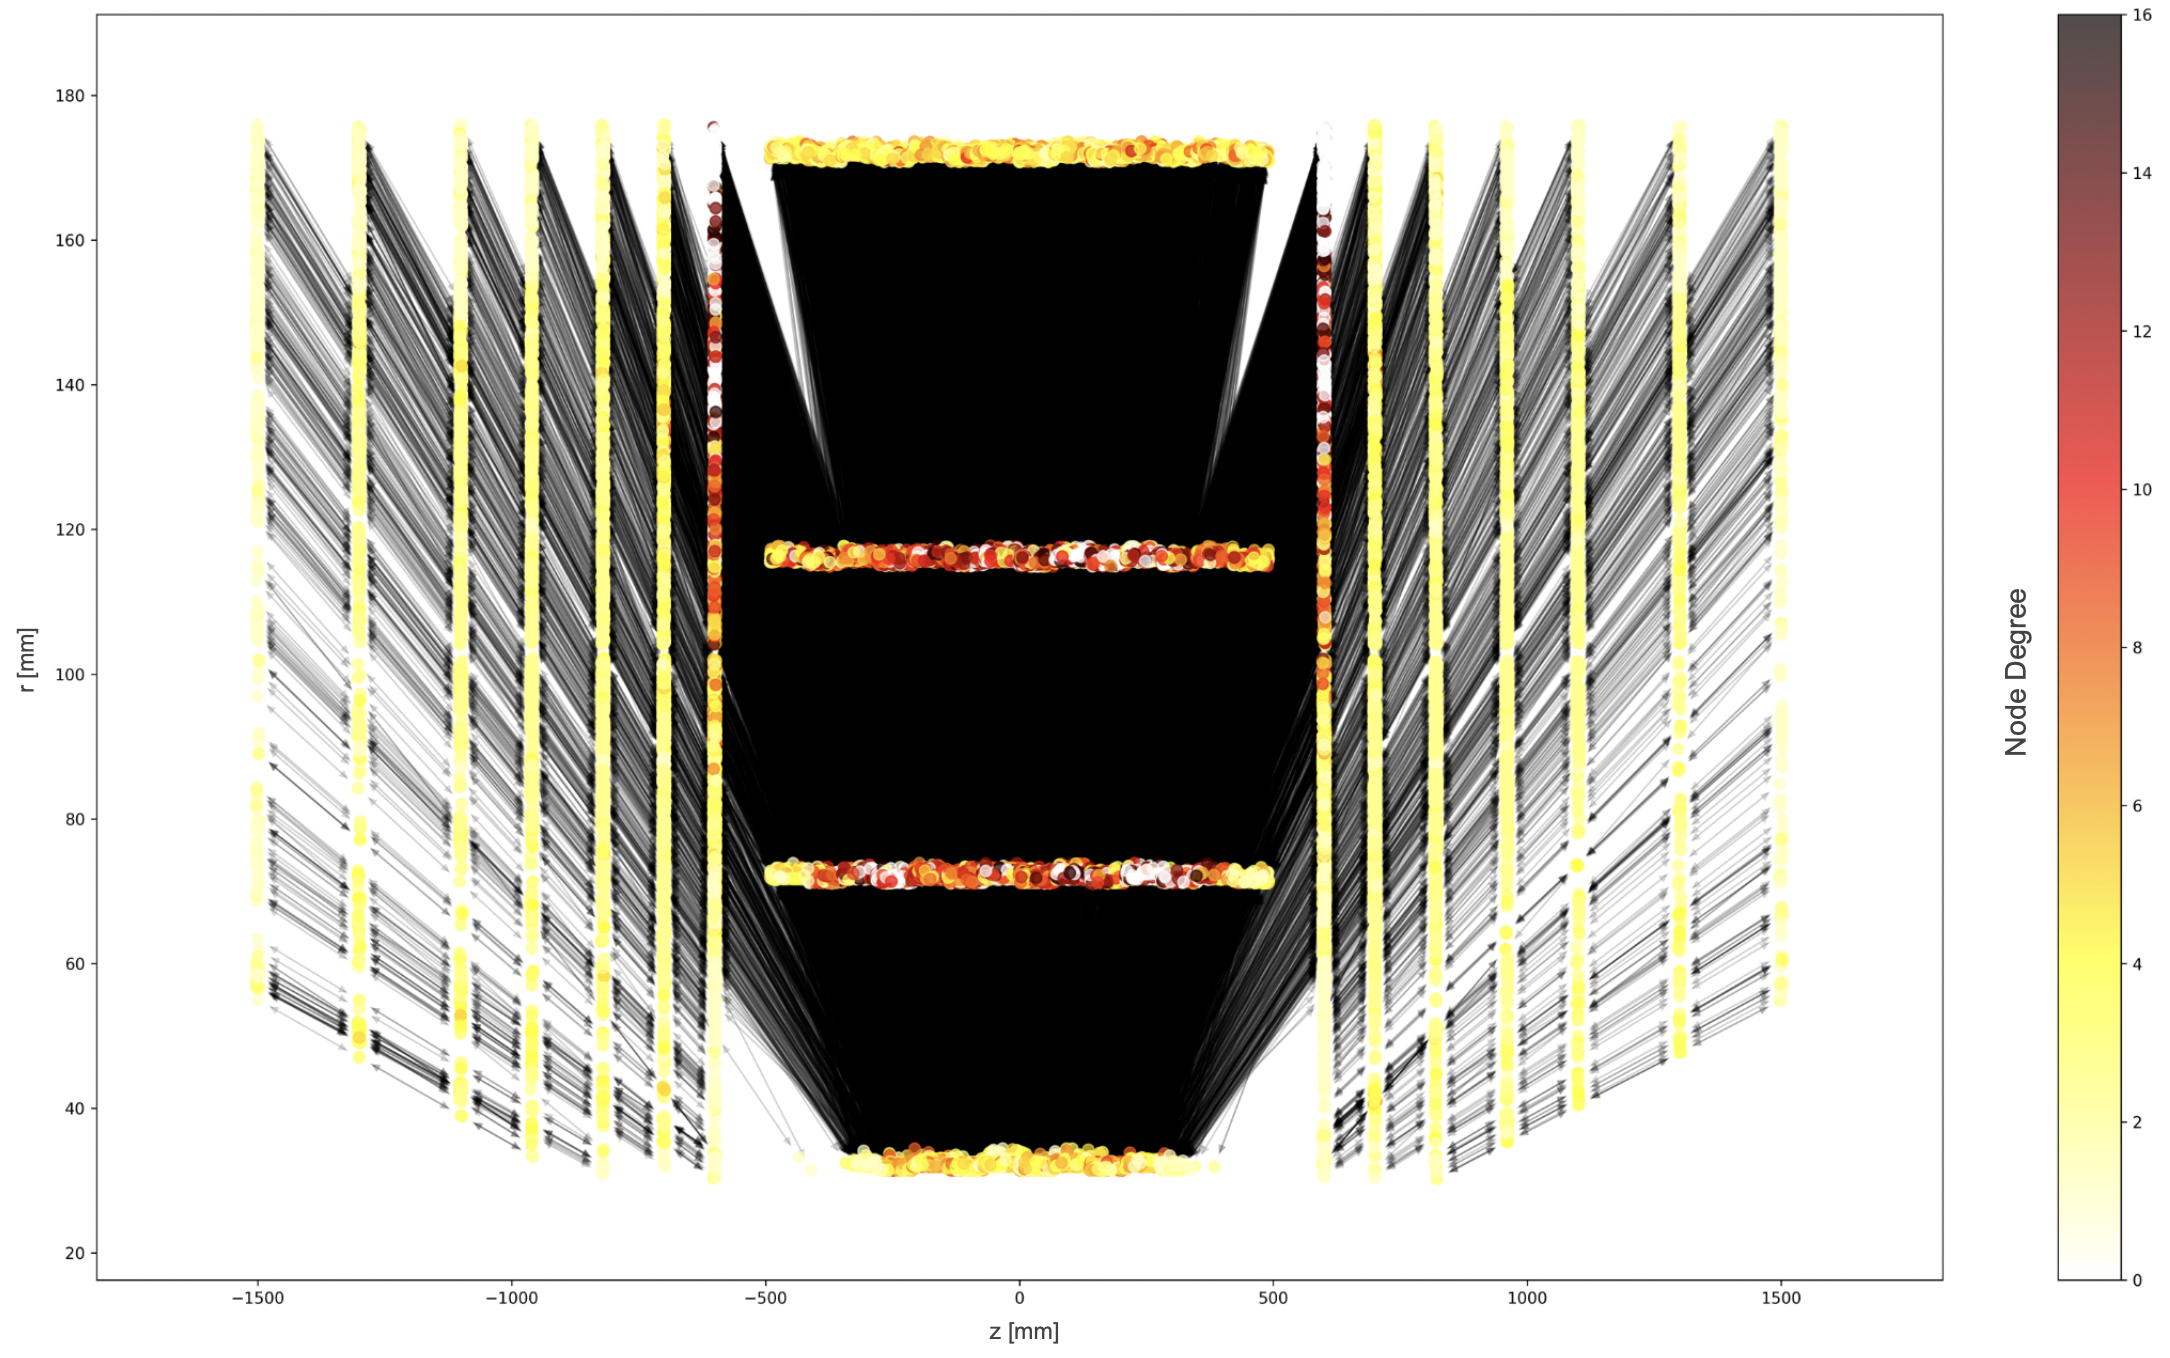
\includegraphics[width=0.99\textwidth]{images/7-results/trackml-barrel-remaining-node-degree.png}
    \caption{TODO: regenerate this plot but with the node degree inverted!!! }
    \label{fig:trackml-results-barrel-endcap-remaining-node-degree}%
\end{figure}




\subsection{Software Optimisations}







\subsection{Other Approaches}
\subsubsection{Community Detection}

%If a subgraph does not meet the criteria to qualify as a good track candidate, a \textit{Community Detection} algorithm \cite{community} is applied in order to further partition the set of nodes. Community Detection is a generalisation of CCA and works by using a distance metric, typically modularity, in order to label nodes as \textit{closely connected}. Modularity is a benefit function that measures the strength of a particular division of a network using the number of edges. A popular modularity maximisation approach is the Louvain method \cite{python_louvain}, which iteratively optimises local communities until global modularity can no longer be improved. An example illustration of a network partition via Community Detection is shown in Figure \ref{fig:community-detection}. Any subgraphs with zero extracted candidates through this procedure are propagated to further stages for additional processing.

%Community Detection: divides nodes into various clusters based on edge structure. It learns from edge weights, and distance and graph objects similarly. 

\begin{figure}[htbp]
   \centering
   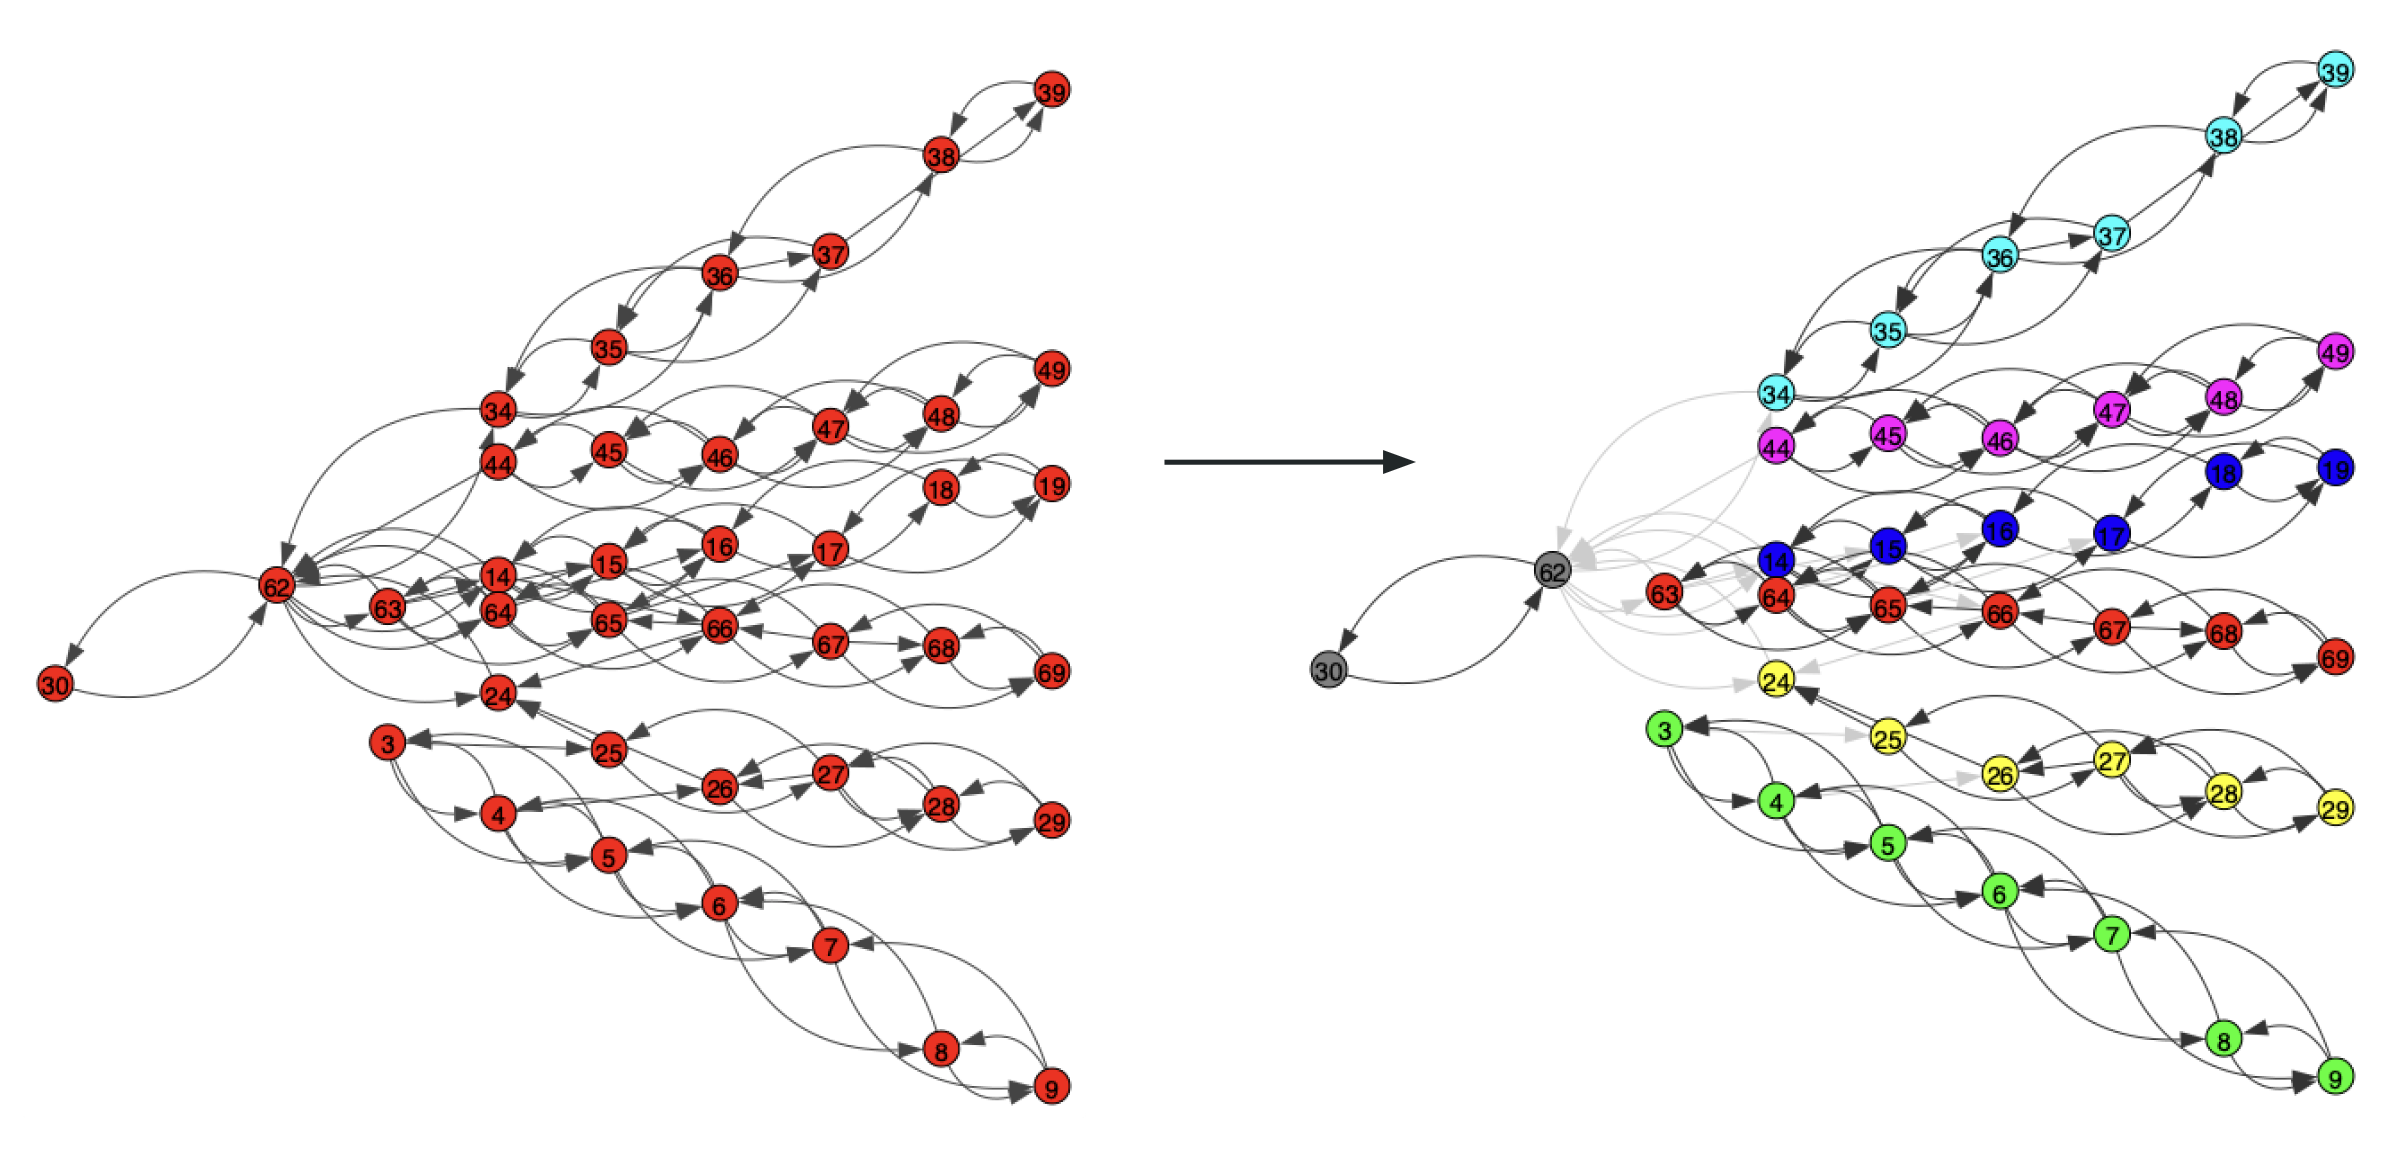
\includegraphics[width=0.99\textwidth]{images/7-results/community-detection.png}
   \caption{TODO: caption ....}
   \label{fig:community-detection}%
\end{figure}

%\begin{itemize}
%    \item extension to barrel, analysis of results, performance  evaluation, challenges and outlook
%    \item Optimisation - GPU acceleration and numpy implementation etc
%\end{itemize}


\section{Conclusion}

% Utilizing message passing to iteratively learn neighbourhood information aids in the pruning of outlier edges within complex regions.

% This key feature of the GNN-based algorithm suggests that the excitation and inhibition rules of individual GNN nodes are designed in such a way to facilitate the “simple-to-complex” approach for “nodes-to-tracks” association. 